 \documentclass[%
    corpo=12pt,
    %twoside,
    stile=classica,
    oldstyle,
%    autoretitolo,
    tipotesi=magistrale,
    english,
    greek,
    evenboxes,
]{toptesi}

%\english
\usepackage{relsize}%           resize used for the "_" character
\usepackage[utf8]{inputenc}%    codifica d'entrata
\usepackage[T1]{fontenc}%       codifica dei font
\usepackage{lmodern}%           scelta dei font
\usepackage{setspace}%          interlinea
{\fontfamily{lmdh}\selectfont
}
%\linespread{1.1} %TODO check this value

\usepackage{colortbl}

\usepackage[table,xcdraw]{xcolor} %colori per intrerno tabelle e altro

\usepackage{float} %useful to use H to fix figures

\usepackage{hyperref}
\usepackage{import}
\hypersetup{%
    pdfpagemode={UseOutlines},
    bookmarksopen,
    pdfstartview={FitH},
    colorlinks,
    linkcolor={blue},
    citecolor={blue},
    urlcolor={blue}
  }
  
%%DEFINING THE RULES FOR THE TABLES
%%commands for the color of the table cells
%%TODO create the color light gray, for the headers
%%TODO create the palettes for the tables
\definecolor{light_gray}{RGB}{205,205,205} %done
\definecolor{llight_gray}{RGB}{225,225,225} %done

\definecolor{azz_palette}{RGB}{190,211,220} %done
\definecolor{gre_palette}{RGB}{234,238,203} %done
\definecolor{yel_palette}{RGB}{245,226,161} %done
\definecolor{ora_palette}{RGB}{232,179,167} %done
\definecolor{pur_palette}{RGB}{217,150,167} %done
\definecolor{pin_palette}{RGB}{248,234,241} %done
\definecolor{red_palette}{RGB}{194,116,116} %done



\definecolor{lazz_palette}{RGB}{222,233,238} %done
\definecolor{lgre_palette}{RGB}{244,245,228} %done
\definecolor{lyel_palette}{RGB}{249,241,207} %done
\definecolor{lora_palette}{RGB}{242,217,210} %done
\definecolor{lpur_palette}{RGB}{235,202,210} %done
\definecolor{lpin_palette}{RGB}{252,245,246} %done
\definecolor{lred_palette}{RGB}{225,186,185} %done



\newcommand{\lgray}{\cellcolor{light_gray}}
\newcommand{\llgray}{\cellcolor{llight_gray}}

\newcommand{\tazzu}{\cellcolor{azz_palette}}
\newcommand{\tgre}{\cellcolor{gre_palette}}
\newcommand{\tyel}{\cellcolor{yel_palette}}
\newcommand{\toran}{\cellcolor{ora_palette}}
\newcommand{\tpur}{\cellcolor{pur_palette}}
\newcommand{\tpin}{\cellcolor{pin_palette}}
\newcommand{\tred}{\cellcolor{red_palette}}



\newcommand{\tlazzu}{\cellcolor{lazz_palette}}
\newcommand{\tlgre}{\cellcolor{lgre_palette}}
\newcommand{\tlyel}{\cellcolor{lyel_palette}}
\newcommand{\tloran}{\cellcolor{lora_palette}}
\newcommand{\tlpur}{\cellcolor{lpur_palette}}
\newcommand{\tlpin}{\cellcolor{lpin_palette}}
\newcommand{\tlred}{\cellcolor{lred_palette}}



  
\usepackage{listings}
%% DEFINING THE RULES FOR THE CODE
\definecolor{vgreen}{RGB}{23,114,69}
\definecolor{vblue}{RGB}{1,127,255}

\definecolor{vorange}{RGB}{255,143,102}
\definecolor{vlightblue}{RGB}{173,216,230}
\lstdefinestyle{verilog-style}
{
    language=Verilog,
    basicstyle=\scriptsize\ttfamily,
    keywordstyle=\bfseries\color{vgreen},
    identifierstyle=\color{black},
    commentstyle=\color{vblue},
    numbers=left,
    numberstyle=\tiny\color{black},
    numbersep=10pt,
    tabsize=8,
    moredelim=*[s][\color{black}]{[}{]},
    literate=*{:}{:}1,
    linewidth=.99\textwidth,
    sensitive = true,
  morekeywords = [1]{
    %% SystemVerilog keywords
    begin,
    bit,
    break,
    case,
    continue,
    default,
    do,
    else,
    end,
    endcase,
    function,
    endfunction,
    endinterface,
    endmodule,
    endpackage,
    enum,
    export,
    extern,
    for,
    if,
    import,
    int,
    interface,
    local,
    localparam,
    matches,
    module,
    package,
    tagged,
    type,
    typedef,
    struct,
    union,
    void,
    %% Bluespec keywords
    property,
    endproperty,
    assert,
    assume,
    bind,
    int,
	task,
	endtask,
	function,
	endfunction,
	input,
	output,
	\$error,
	\$fatal,
	\$isunknown,
	new,
	class,
	endclass
  },
}
  
  
  
  
  
 
  
  

\ExtendCaptions{english}{Abstract}{Acknowledgements}
\newcommand{\+}{\textscale{.5}{\textunderscore}}

\begin{document}\errorcontextlines=9
\english
%%%%%%% Questi comandi è meglio metterli dentro l'ambiente
%%%%%%% ThesisTitlePage con o senza asterisco, oppure in un file di
%%%%%%% configurazione personale. Si veda la documentazione
%%%%%%% inglese o italiana.
%%%%%%% Comunque i presenti comandi servono per comporre la
%%%%%%% tesi con i moduli di estensione standard del pacchetto
%%%%%%% TOPtesi.

\begin{ThesisTitlePage}

% Per cambiare la dicitura sopra la lista dei laureandi decommentare
% la riga seguente, cambiando le 4 parole in modo consistente
%
\TitoloListaCandidati{Candidate:, Candidate:, Candidates:, Candidates:}
%
\ateneo{Politecnico di Torino}


%
% Non tutte le università hanno un nome proprio
%\nomeateneo{}
%
\struttura[III]{Matematica, Fisica e~Scienze Naturali}
%\Materia{Remote sensing}
\titolo{Functional and Formal Verification on submodules of a Vector Processing Unit based on RISC-V V-extension}% per la laurea quinquennale e il dottorato
%%%%%%% Logo della sede
\logosede{LOGO_2.png}% 

%
%%%%%%% Corso degli studi
\CorsoDiLaureaIn{Master's Degree in}
\corsodilaurea{Electronic Engineering}% per la laurea

\TesiDiLaurea{Master's Thesis}
\AdvisorName{Supervisor:}
\CoAdvisorName{Cosupervisors}

%%%%%%% L'eventuale numero di matricola va fra parentesi quadre
%\show\Candidato
%\def\Candidato{Studente}
%\show\Candidato
\renewcommand*\IDlabel{\\\quad ID:\space}
\candidato{\textsc{Guglielmi} Vito Luca }[s265044] 
%\secondocandidato{Evangelista \textsc{Torricelli}}[123457]

%%%%%%% Relatori o supervisori
%
    \relatore{Prof.~\textsc{Lavagno} Luciano}
    \secondorelatore{Prof.~\textsc{Moll Echeto} Francesc}
    \terzorelatore{Dr.~\textsc{Palomar} Oscar}
% 
%%%%%%% Per mettere altri relatori consultare toptesi-it.pdf

%%%%%%% Tutore
%\tutoreaziendale{}
\NomeTutoreAziendale{Barcelona Supercomputing Center}

%%%%%%% Seduta dell'esame
%\sedutadilaurea{Agosto 1615}
%%%%%%%% oppure:
\sedutadilaurea{\textsc{October} 2020}% 


\end{ThesisTitlePage}


%%%%%%% Per cambiare l'offset per la rilegatura;
%%%%%%% meno offset c'e', meglio e'
%\setbindingcorrection{3mm}

\begin{dedica}
    \normalsize{Alla mia famiglia.}
\end{dedica}

\newpage

\summary
\english

This thesis was developed while working at Barcelona Supercomputing Center, a research center specialized in High Performance Computing and investigation in many fields, such as cloud computing, bioinformatics, material science and more.\\


Taking part to European Processor Initiative (EPI) project, the whole thesis aims to perform the verification process on a Vector Processing Unit.
The implemented Vector Processing Unit is based on the RISC-V V-Extension, which is a set of specifications defining the Instructions Set Architecture (ISA) of a vector core. The V-Extension is currently on develop by the RISC-V foundation. This manuscript will refer to the versions 0.7.1.\\

The   first  chapter consist of an introduction of the needed concepts and of the context in which this thesis is been developed.\\

Then, in the second chapter, all the techniques used to verify functionally and formally this VPU are discussed.\\

All the results, such as found bugs or created material, are displayed in the third chapter. Moreover, analysing these results, the efficacy of the techniques used is evaluated. It is shown how formal and functional tools can be used to find bugs or to better define specification. \\

In the last chapter, it is possible to conclude that the techniques  adopted produced the expected results showing significant improvements in the verification effort.








\bigskip



\tableofcontents
\clearpage
\mainmatter


\chapter{Introduction}
This thesis is based on part of the EPI-project, developed at Barcelona Supercomputing Center, in particular on the V-Extension implementation.
In this Chapter there will be presented and discussed all the RISC-V and V-Extension concepts, but they will be not covered all the topics regarding the RISC-V ISA or all the extensions, as they are not always relevant to the project.\\
Starting from the Concepts there will be also an explaination on the context of the project, so the real implementation and application of the ISA specifications.
In particular there will be a exposition of Verification concepts and on the UVM structure, filled by the details useful to understand the work done.



\section{Concepts}
\subsection{RISC-V}
RISC-V is an open, extensible and free instruction set architecture (ISA). It was originally designed to support computer architecture research and education\cite{RISC-V-Instruction-Set-Manual}.\\
The project began at the Berkley, University of California in 2010, and then in 2011 was published the first ISA User Manual. After that there was the first tapeout of a RISC-V chip in 28nm FDSOI donated by STMicroelectronics.\\

The RISC-V ISA is implemented as a base integer ISA, but it is modular and so supports  variable-length instruction encodings.\\
This ISA is provided under open source licenses, and it is gaining a lot of popularity due to its open nature. \\
Mainly there are two primary base integer variants, RV32I and RV64I, which provide 32-bit or 64-bit user-level address spaces respectively.\\

RISC-V is designed to have good customization and so it's provided with the possibility to be extended, but the base integer instructions cannot be redefined.\\
There are two kinds of extensions:
\textit{standard} and \textit{non-standard}.
\begin{itemize}
    \item The \textit{standard} ones need to be compatible with all the other standards and also they should aim to be generally useful.
    \item The \textit{non-standard} ones can be highly specialized in some task and so can be in conflict with other extensions.
\end{itemize}

For general development some standard extensions are predefined:
\begin{itemize}
    \item "\textbf{I}" is the base integer extension and contains integer computational instructions, integer loads, integer stores, and control-flow instructions. It is mandatory for all RISC-V implementations.
    
    \item "\textbf{M}" is the standard integer multiplication and division extension, it allows to multiply and divide the values held in the integer registers.
    
    \item "\textbf{A}" is the standard atomic instruction extension. For inter-processor synchronization is useful to have atomic instructions so with this extension is possible to read, modify, and write memory atomically . 
    
    \item "\textbf{F}" is the standard single-precision floating-point extension. It adds floating-point registers, single-precision computational instructions, and single-precision loads and stores. 
    
    \item "\textbf{D}" The standard double-precision floating-point extension. It is useful when the F extension is not enough, so expands it and adds double-precision computational instructions, loads, and stores.
    
    \item "\textbf{G}" is the denotation for an integer base plus these four standard extensions (“IMAFD”).
\end{itemize}


The design philosophy of the RISC-V projects is based on modularity: the base ISA will not change over time, but new extensions will be available and new feature will be added. This is useful because is very difficult to find general useful extension beyond the ones already exist. So it wouldn't be convenient to constantly add new features to the base ISA and then have to keep track of that.\\
In Figure \ref{riscv-base-instruction-formats} it is possible to see how the base instruction are composed.

\begin{figure}[H]
    \centering
    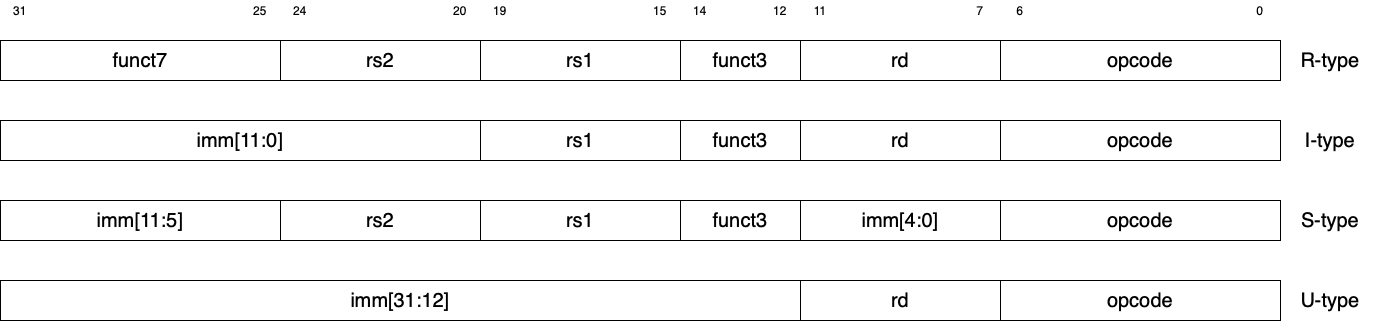
\includegraphics[scale = 0.27]{Chapter_1/img/riscv-base-instruction-formats.png}
    \caption{RISC-V base instruction formats. \cite{RISC-V-Instruction-Set-Manual}}
    \label{riscv-base-instruction-formats}
\end{figure}

It is important to notice that RISC-V is a load-store architecture, this means only load and store operations can have access to the memory.\\
It is a very convenient organization, because it reduces the average time-per-operation and guarantees a good functioning of the pipelined structure.\\

It also supports signed byte and half word loads, which is very useful when  working with signed byte and half word data types.

In Figure \ref{riscv-load-store} it is possible to see how the load-store instructions are composed, and that the LOAD is a I-type op and the STORE is an S-type op.

\begin{figure}[H]
    \centering
    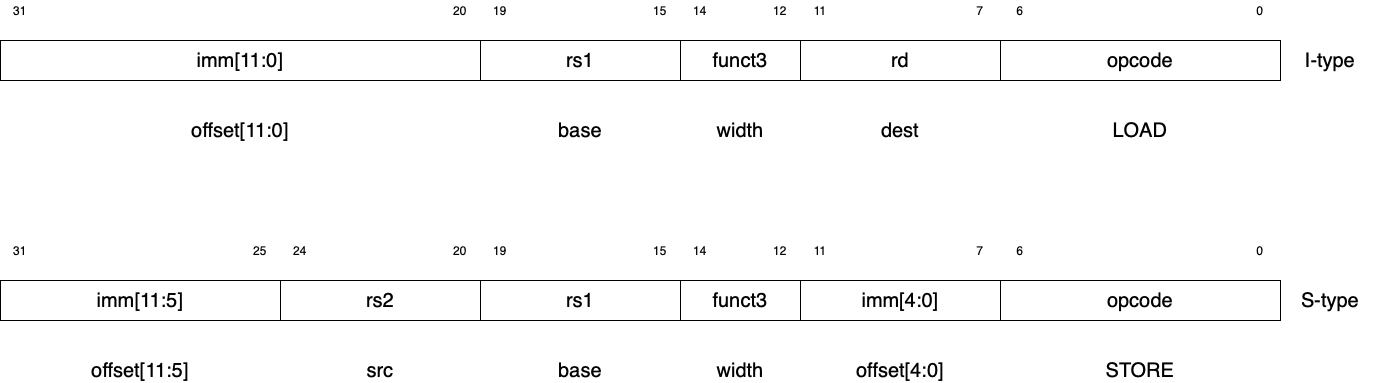
\includegraphics[scale = 0.27]{Chapter_1/img/riscv-load-store.png}
    \caption{RISC-V load/store instruction formats. \cite{RISC-V-Instruction-Set-Manual}}
    \label{riscv-load-store}
\end{figure}


\subsection{Parallel architectures, Vectors and RISC-V V-Extension}
In the last years the parallel architecture are gaining inertia on the processors field. This is happening because the real world has parallel behaviour and so the hardware we use to compute simulations and calculus needs to be.\cite{Parallel-Computing}\\
But why now and not before?\\
In the past, parallel computing efforts have shown promise and gathered investment, but in the end, uniprocessor computing always prevailed, what is different now?\\
Well, most of the paradigms that led to the unicore decision are now changing quickly as the technology changes its needs.\\
As the technology scales down to the nanometers, the power consumption and the energy consumption are becoming a problem, instead the cost of a single transistor is significantly lower.\\

But the multicore solution still doesn't meet the conformity for old binaries compilations and it could be difficult to program. So the solution of a parallel architecture with "manycores" seems to be the right one.\\

For this reason the vectors are useful. They allow to compute data in a parallel way, without having multicore programming logic.\\
A classic example are the VPU (Vector Processing Units) working with SIMD (single instruction multiple data).\\

A famous example of a vector architecture is the Cray-1. It was presented in 1975, and was a load/store architecture, as seen before.
It was designed for Supercomputing and the major feature was to have also a scalar mode. This because the vector computation is not always useful.\\

As it is possible to see in Figure \ref{Multithreading} with standard multithreading there will always be some empty thread along with the running ones. This lowes the efficiency.
\begin{figure}[H]
    \centering
    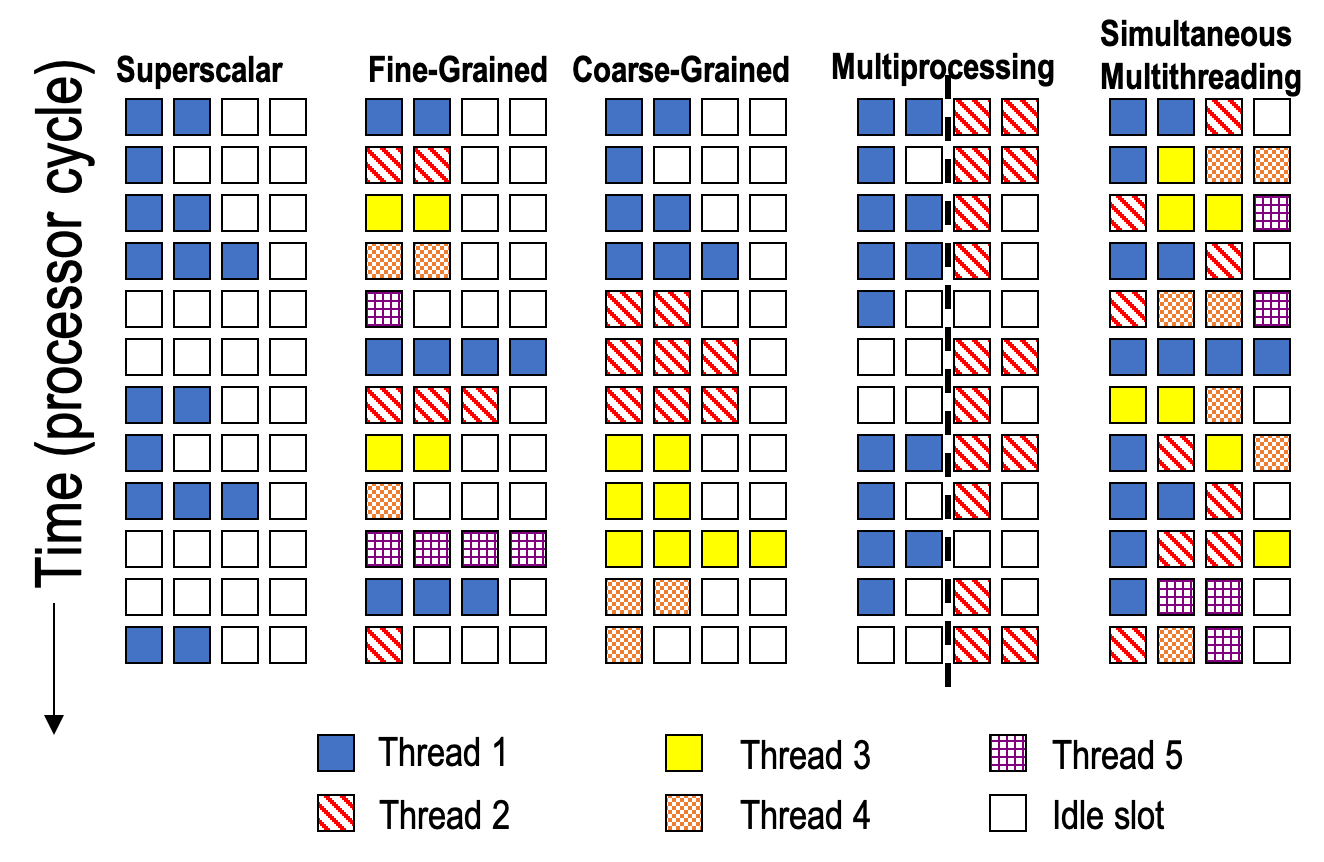
\includegraphics[scale = 0.4]{Chapter_1/img/multithreading.png}
    \caption{Multithreading Processor Clock Time usage  \cite{L15-Krste}}
    \label{Multithreading}
\end{figure}

Indeed the major advantage with the Vector computation is the condensation of the processor usage. 
So the usage will not be distributed as for standard multithreading processors, but it will have full usage for some cycles and zero usage for others\cite{L15-Krste}.\\

But of course there is a drawback, in particular the Latency. In vector computing there are always some dead cycles, but this also allows to increase the efficiency with modern low-power techniques, if it is possible to decrease the energy usage during the dead time.
The pipeline is represented in Figure \ref{Vector-Latency} and the final Clock Tima usage is represented in Figure \ref{Vectoring}.

\begin{figure}[H]
    \centering
    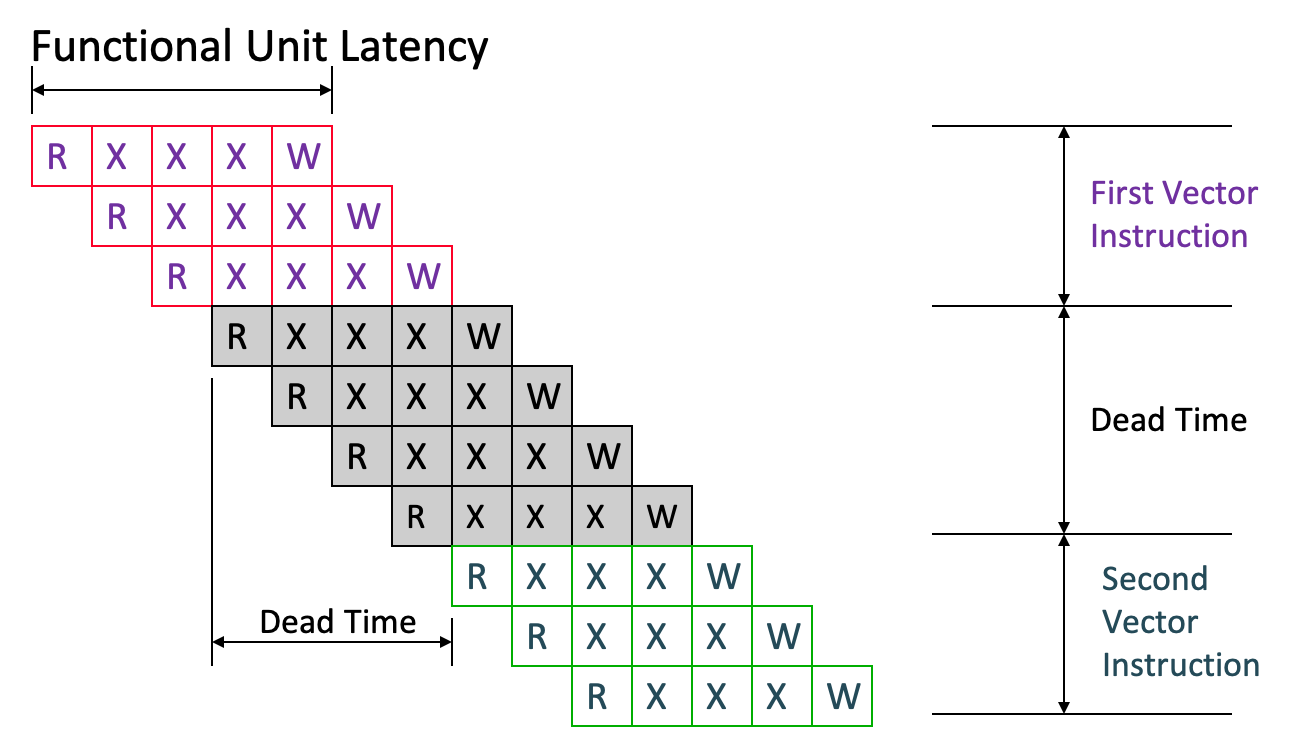
\includegraphics[scale = 0.4]{Chapter_1/img/vectoring.png}
    \caption{Latency penalty on vector processing units \cite{L15-Krste}}
    \label{Vector-Latency}
\end{figure}

\begin{figure}[H]
    \centering
    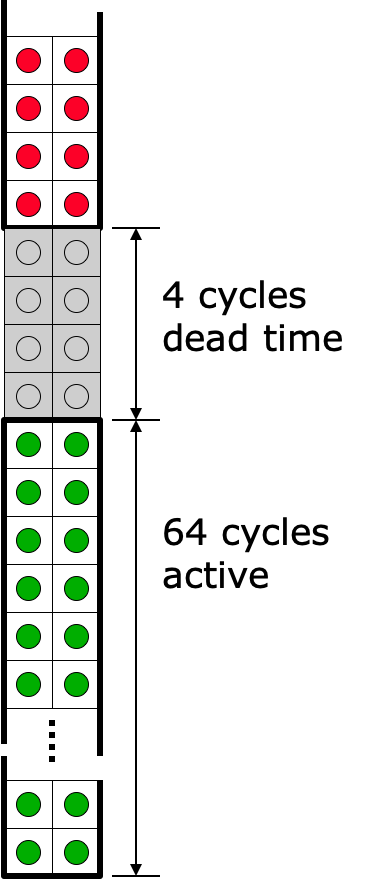
\includegraphics[scale = 0.4]{Chapter_1/img/vectoring_2.png}
    \caption{Vector Processor Clock Time usage \cite{L15-Krste}}
    \label{Vectoring}
\end{figure}
The RISC-V solution is V-Extension (V stands for Vector), and is in current development, in this thesis the reference will be the V-Extension 0.7.1.

The vector extension adds 32 vector registers, and five unprivileged CSRs (vstart, vxsat, vxrm, vtype, vl) to a base scalar RISC-V ISA\cite{riscv-v-specs}.
There are also 8 vector predicate registers (vp0-vp7). The CSRs vectors define the configurations.

\begin{table}[H]
    \centering
    \begin{tabular}{|l|l|l|l|}
        \hline
        Address & Privilege & Name   & Description               \\ \hline
        0x008   & URW       & vstart & Vector start position     \\ \hline
        0x009   & URW       & vxsat  & Fixed-point Saturate Flag \\ \hline
        0x00A   & URW       & vxrm   & Fixed-Point Rounding Mode \\ \hline
        0xC20   & URO       & vl     & Vector length             \\ \hline
        0xC21   & URO       & vtype  & Vector data type register \\ \hline
    \end{tabular}
    \caption{RISC-V's CSRs}
    \label{CSRs}
\end{table}

Based on the base scalar ISA and on the extensions implemented the datatypes and operations supported by the V extension change and they can be 16-bit, 32-bit, 64-bit, and 128-bit floating-point types or fixed-point types (F16, F32, F64, and F128, or X8, X16, X32, X64, and X128 respectively) \cite{riscv-v-specs}.\\


The vector unit must be configured before use. 
The active vector length is held in the CSR vl, which can only hold values between 0 and MVL inclusive.
The active vector length is usually written with the setvl instruction.\\

Other than the base instruction we can expect from a Vector Architecture (as a move, add, xor and so on) it is possible to find some useful operations related to the nature of the vector calculus\cite{riscv-v-specs}:
\begin{itemize}
    \item \textbf{vectorial load/store}: those can strided or indexed. The strided ones index the elements referring to a starting one and then adding (or subtracting) a certain stride. This kind of load/store is very fast, in particular in some special cases (as unit-strided or some optimized power of 2).\\
    The elements into the indexed ones are basically pointed with an index. This process really slows down the operation but allows to select directly the elements.
    
    \item \textbf{widening/narrowing}: those operation are used to increase or decrease the size of the vector's contents, in fact they are very useful when performing operations that need to increase the result size (as example a multiplication between to integer at 32 bit needs to have 64 bit to not loose information). There are also few operations that require the inverse resizing, so the narrowing.
    
    \item \textbf{gather}: those are very particular operations and very useful when manipulating vectors. They allow to index a vector using another vector as index. In this way various patterns are possible.
    
    \item \textbf{reduction}: finally the reduction can perform an operation between a scalar and a vector and give as result a scalar (an easy example could be to calculate the maximum value between all the value contained in a vector and one scalar, the result would either be one of the element of the vector or the scalar).
    
\end{itemize}


Finally all those operations can be \textit{masked}. The masking is a common operation when there is branching or when complex patterns emerge.
Normally one bit of the mask represent a whole work or byte into the vector. Then an AND op is performed to have the final result. 

\subsection{Verification}
As the technology scales down, the design complexity explodes. 
Very small form factor have conflicting requirements for high performance, low-power and area constraints. 
This lead to a complex design and to elevate the costs of it.\\

It is possible to see in Figure \ref{verification-tecnology} how the cost for verification increases drastically with the lowering of the technology node.


\begin{figure}[H]
    \centering
    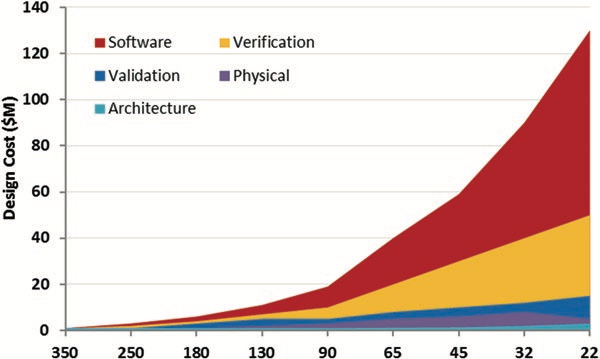
\includegraphics[scale = 0.6]{Chapter_1/img/verification-tecnology.png}
    \caption{Verification cost vs technology node \cite{verification-book-2018}}
    \label{verification-tecnology}
\end{figure}

the verification is responsible to make sure the design is in track with the specification, so as the design complexity increases so does the verification.\\

This is of course an issue for the time-to-market. 
In particular functional design verification takes 40–50\% of the project resources. In other words, increase the productivity of functional design verification and shorten the design / simulate / debug / cover loop is an essential task \cite{verification-book-2018}.\\

Also the compounded complexity grows faster that the compounded productivity. This gap only means the verification needs to be faster and so need to implement more techniques.
It is possible to see a study on the complexity/productivity gap in Figure \ref{complexity-gap}
\begin{figure}[H]
    \centering
    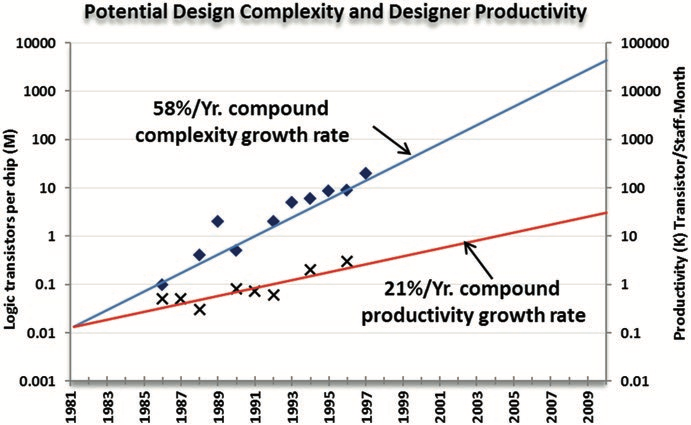
\includegraphics[scale = 0.5]{Chapter_1/img/complexity-gap.png}
    \caption{The gap between the complexity and the productivity \cite{verification-book-2018}}
    \label{complexity-gap}
\end{figure}


The verification mainly is divided in Functional and Formal verification:
\begin{itemize}
    \item \textbf{Functional}: it need to verify if the functionalities described into the specifications are met into the design. To verify functionally it is needed to define the functionalities and write them as code (normally checkers or scoreboard). This is a very important part of the process, as this translation is never perfect and often highlights some critical point into the specs.
    
    \item \textbf{Formal}: the formal verification can be done in different ways as \textit{model checking}, \textit{equivalence checking} and \textit{theorem proving}. \textit{Theorem proving} tries to prove the equivalence between specs and design using mathematical reasoning. \textit{Model checking} is useful when performing optimization to the design, trying to demonstrate the various versions are mathematically equivalent. Finally the \textit{model checking} is used to try to find counter example on the behaviour of the design, and in case simulating the specific case to demonstrate the falsity.
\end{itemize}

\bigskip


The whole process of verification need also to have a direction. For that is used Coverage. \\

Coverage is very useful and can be performed on functionalities or on the code:
\begin{itemize}
    \item functionality: it measure the cover of all the functionalities stated by the specs. In this way it is possible to assure all the requirements are met. But this also means there is no information about not used RTL.
    
    \item code: it measure the cover of all the code. This means it is possible to know if there is unused code and possibly some branch of the flow. This also means there is no check about the functionalities implemented.

\end{itemize}

Trying to take the coverage to 100\% is the main goal. But at the same time it is easy to fool the coverage. This because it depends on how the cases are taken into account. \\

To be able to use all those techniques there is the need of a structure to contain and control them.
This structure is called \textit{UVM}, and it is formed by different classes useful to instantiate the controls and the drivers needed to verify the RTL. It will be discussed the particular case of this work later on this Chapter.

\section{Context}
\subsection{The VPU}
\begin{figure}[H]
    \centering
    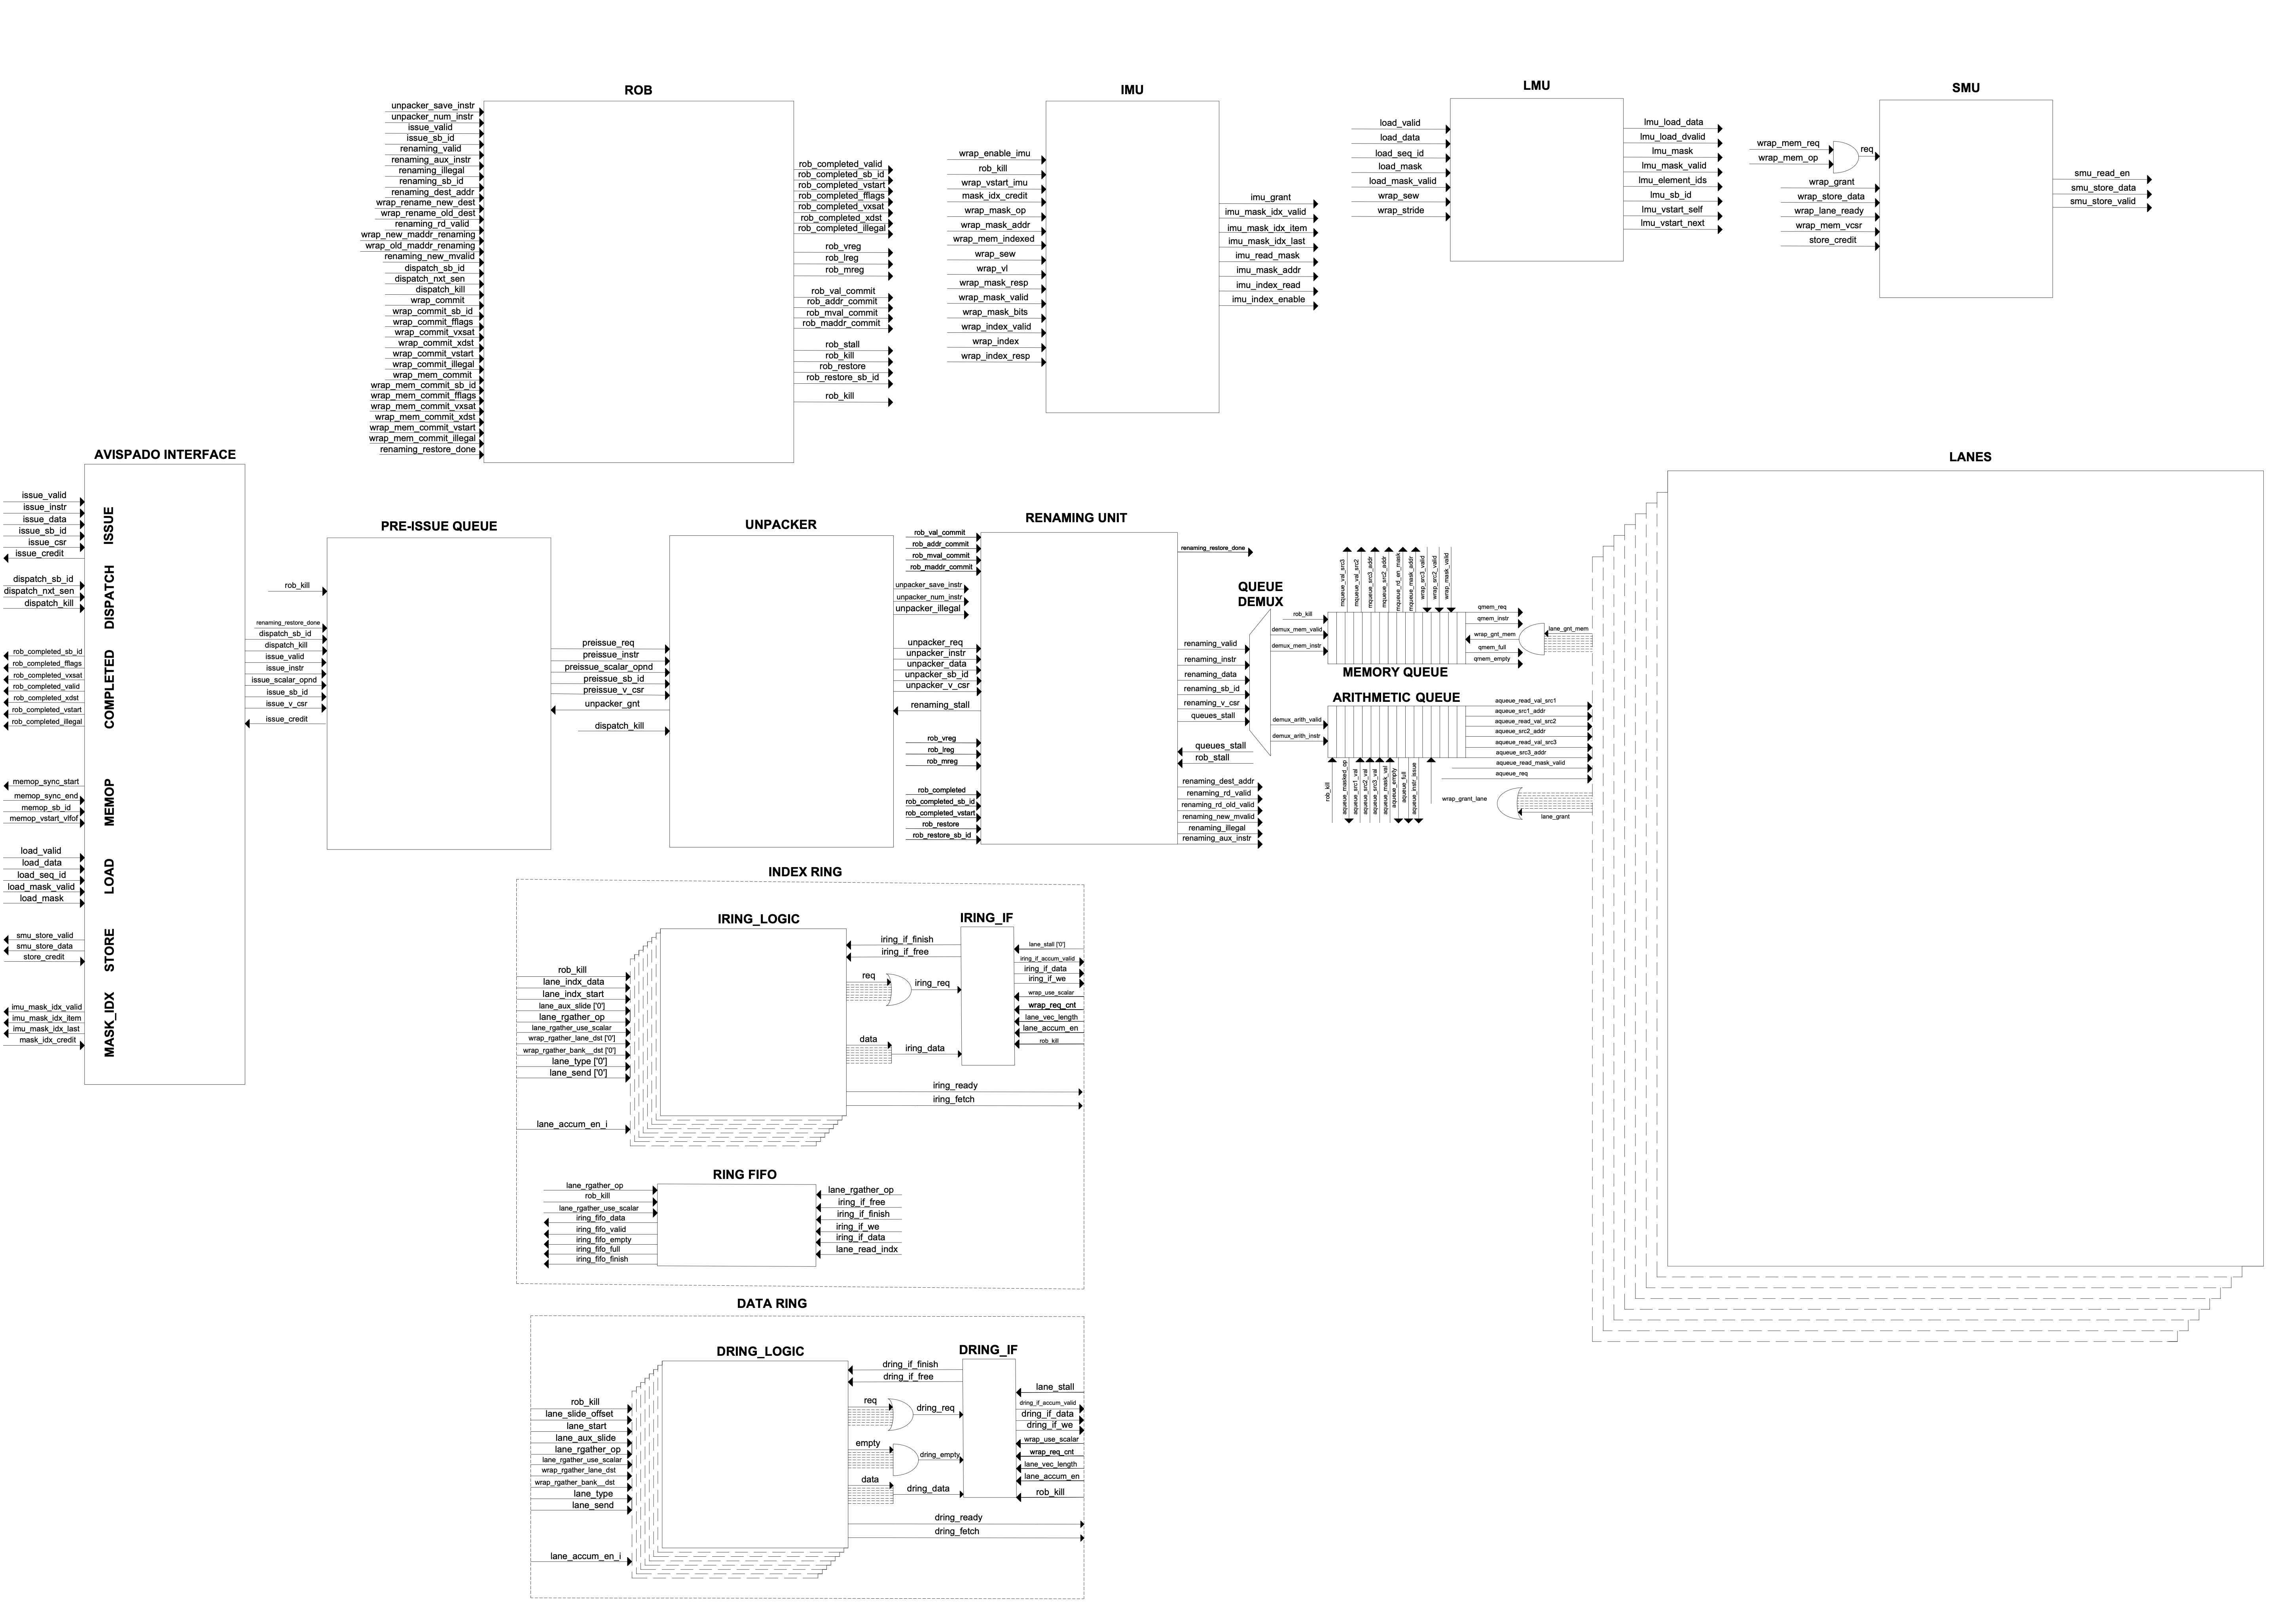
\includegraphics[scale = 0.07]{Chapter_1/img/VPU-wo-LANE.jpg}
    \caption{EPI project's VPU}
    \label{VPU-wo-LANE}
\end{figure}
%%images by victor, take the google drive infos

\subsection{Submodules}
%description on LB and LMU mainly and on the checkers in generale

\subsection{The UVM and the checkers}
%%the all draw in to the wiki and the main description of every piece would be great.


\chapter{Contributions}
Most of the code created to verify the design was written in SystemVerilog. This is a hardware description language, created as an evolution of the Verilog language, adding some extensions as OOP and specific keywords for assertions and coverage.
Other languages were used for the scripting as Python and tcl.


\section{Submodules and Specifications}
%%talk about the specs


The main focus of this thesis will be on two important submodules in charge of their load instructions:

\textit{Load Buffer} and \textit{Load Management Unit}.

\subsection{Load Management Unit}
%general


This module is in charge of handling the load operations. It receives cache lines from Avispado containing the data for the load. Then, the LMU rearranges the data to distribute it to the vector lanes.
Those can be strided or indexed.

Since the VPU is able to work out-of-order and with two loads in parallel, an ID system is necessary, so each instruction comes with an ID.
In particular the load operation come with the signal \textbf{seq\+id\+i}.
This signal identifies the load and contains all the determinant informations about it.

The main elements of this submodules are:
\begin{itemize}
    \item \textit{Shifter}: it is useful to have the first bit not in the MSB or LSB position.
    
    \item \textit{Compactor}: it is useful to compact all the valid elements. When the stride equals one there is no use of the compactor.
    
    \item \textit{Aligner}: it is in charge to align the elements for the output (lane, bank and sub-bank).
\end{itemize}

\bigskip

%params
The main parameters defining this submodule are:
\begin{itemize}
    \item \textbf{MEM\+DATA\+WIDTH}: width of the chunk of data received from Avispado. The standard value is \textit{512}.
    
    \item \textbf{SEQ\+ID\+WIDTH}: width of the \textit{seq\+id\+i} that identifies the data coming from Avispado. The standard value is \textit{33}.
    
    \item \textbf{MAX\+NUMBER\+ELEMENTS}: maximum number of elements that can be encoded in the chunk of data received (64 when SEW = 8 bit). The standard value is \textit{64}.
    
    \item \textbf{MAVISPADO\+LOAD\+MASK\+WIDTH}: Indicates the maximum number of mask bit that are received with the data. Every bit of the mask represents a byte into the data. The standard value is \textit{64}.
    
    \item \textbf{NUM\+LANES}: number of lanes. The standard value is \textit{8}.
\end{itemize}

\subsubsection{Interface}
%interface
%%%%%%%%%%%%%%%%TABLE%%%%%%%%%%%%%%%%%%%%%%%

\begin{table}[H]
\centering
\begin{tabular}{|l|l|}
\hline
\rowcolor[HTML]{EFEFEF} 
\multicolumn{1}{|c|}{\cellcolor[HTML]{EFEFEF}Signal} & \multicolumn{1}{c|}{\cellcolor[HTML]{EFEFEF}Description}                      \\ \hline
load\+granted\+i    & a load is granted,\\
                    & it will have a certain sew\+i and stride\+i\\ \hline
load\+granted\+sb\+id\+i    & the id for the issued Load,\\
                            & can be issued up to 2 loads\\ \hline
indexed\+load\+granted\+i   & the granted load is indexed \\ \hline
load\+sync\+end\+i          & indicates if the load is ended\\ \hline
load\+sync\+end\+sb\+id\+i  & indicates the load id of the ended load\\ \hline
load\+data\+valid\+i        & indicates if the data in load\+data\+i bus is valid\\ \hline
load\+data\+i               & data received from Avispado\\ \hline
seq\+id\+i                  & the sequence id (described below)\\ \hline
mask\+valid\+i              & validity of mask\+i signal\\ \hline
mask\+i                     & mask bit to mask load\+data\+i\\ \hline
sew\+i                      & identifies the size of each vector element\\ \hline
stride\+i                   & stride indicated in bytes\\ \hline
load\+data\+o               & output data sent to the lanes\\ \hline
load\+dvalid\+o             & indicates if the data in load\+data\+o bus is valid\\ \hline
mask\+o                     & mask bit to mask load\+data\+o\\
                            & it is needed also for not masked inst.\\ \hline
element\+ids\+o             & identifies each element sent in load\+data\+o\\ \hline
sb\+id\+o                   & identifies the instruction\\ \hline
vstart\+self\+o             & identifies the first valid element\\
                            & in the chunk of data received in load\+data\+i\\ \hline
vstart\+next\+o             & identifies the last valid element \\
                            & in the chunk of data received in load\+data\+i\\ \hline
min\+element\+id\+idx\+o    & index of the first valid \\
                            & element in elements\+ids\+o of each lane.\\ \hline
\end{tabular}
\end{table}


\subsubsection{Sequence ID}
The sequence id ID is necessary as the memory system does not guarantee the in-order arrival of elements. So this signal contains all the info needed to correctly elaborate the data.\\

It is composed as:
\begin{itemize}
    \item \textbf{seq\+id\+i[4:0]} = \textit{v\+reg}, identifies the logical vector register that the data should be written to;
    
    \item \textbf{seq\+id\+i[15:5]} = \textit{el\+id}, identifies the lowest valid element id contained in the chunk of data being transmitted;
    
    \item \textbf{seq\+id\+i[21:16]} = \textit{el\+off}, identifies the offset in the chunk of data being transmitted.
    
    \item \textbf{seq\+id\+i[28:22]} = \textit{el\+count}, identifies the number of valid elements being transmitted. Masked elements are valid elements; 
    
    \item \textbf{seq\+id\+i[32:29]} = \textit{sb\+id}, sb\+id of the load instruction that requested the data.
\end{itemize}


\subsubsection{Handshake}
The handshake protocol with the different components is as important as the data manipulation. Following, there is a simple example with stride equal to 1 and offset = 0 (so, no manipulation on the data in input).

\begin{enumerate}
    \item Up to 2 load are granted from the Memory Unit with the load\+granted\+i signal, and the information of SEW and stride of the relative instruction are passed;
    
    \item Avispado sends the data and the seq\+id\+i with its seq\+id;
    
    \item The next clock cycle the data is on the output for the Vector Lane;
    
    \item When a load is finished, another load can be granted.
\end{enumerate}

\begin{figure}[H]
    \centering
    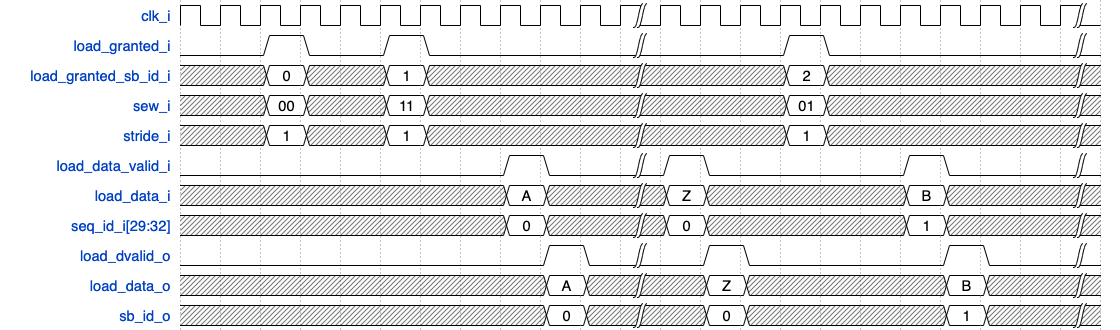
\includegraphics[scale = 0.35]{Chapter_2/img/lmu-time.png}
    \caption{Timing Diagram unit-strided load for the LMU}
    \label{lmu-time}
\end{figure}

In Figure \ref{lmu-time} it is possible to see an example for a unit-strided load. This is a simple load, and its behaviour will be discussed in the following section.

\subsubsection{Strided Load}
In this case all the valid elements are separated by a constant stride. If the stride is equal to 1, then it is called unit-stride.\\

Figure \ref{lmu-strided} shows how the LMU works in this case.\\
The parameters (defined in the seq\+id\+i) are defining the elements to consider.
\begin{figure}[H]
    \centering
    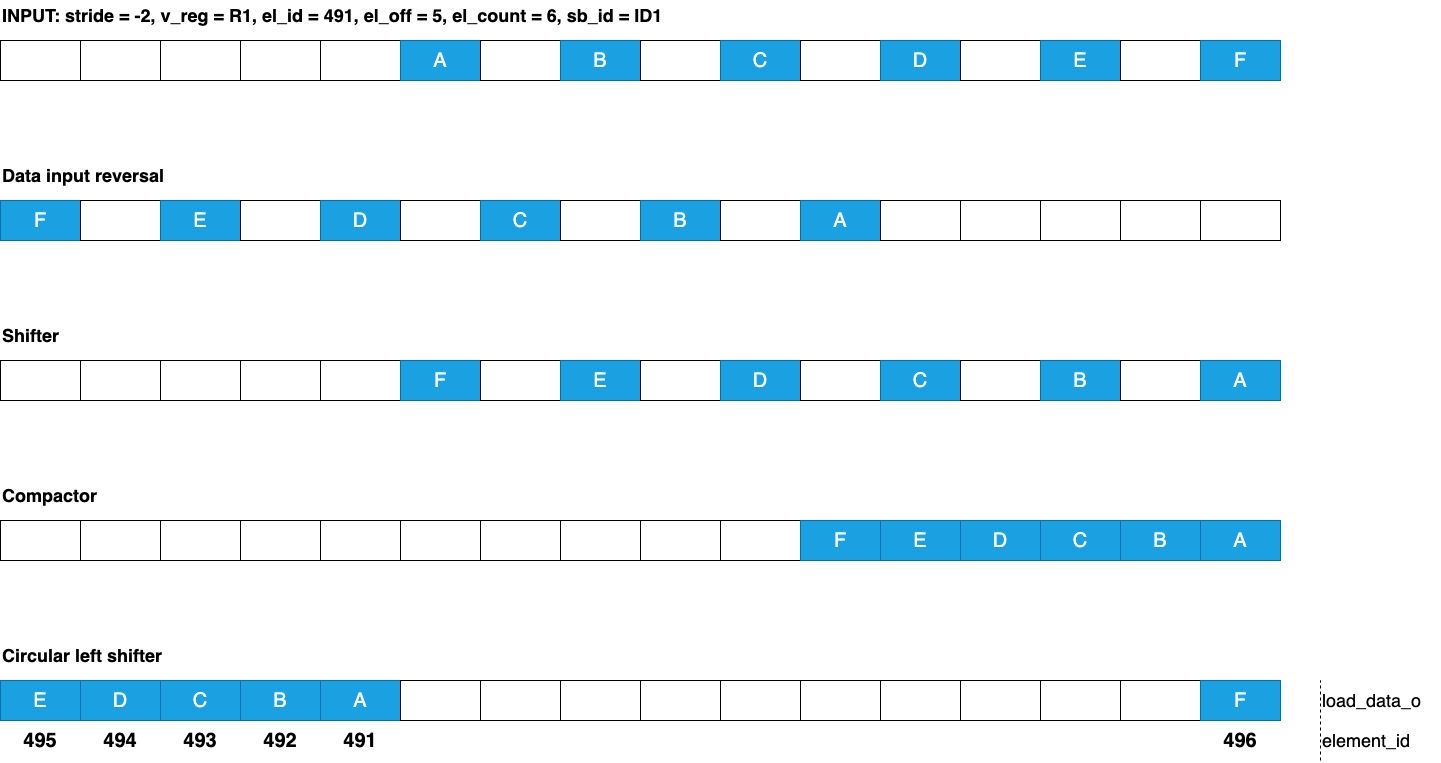
\includegraphics[scale = 0.25]{Chapter_2/img/lmu-strided.png}
    \caption{Strided load handled by the LMU}
    \label{lmu-strided}
\end{figure}

\subsubsection{Indexed Load}
It is also possible to load values in an indexed way. By design was chosen that only one valid element at time is sent, and so el\+count needs to be = 1. If the indexed load is performed with many valid elements, the cache lines is sent multiple times with only one valid element each time.\\

In Figure \ref{lmu-indexed} it is possible to see an example for a simple indexed load.

\begin{figure}[H]
    \centering
    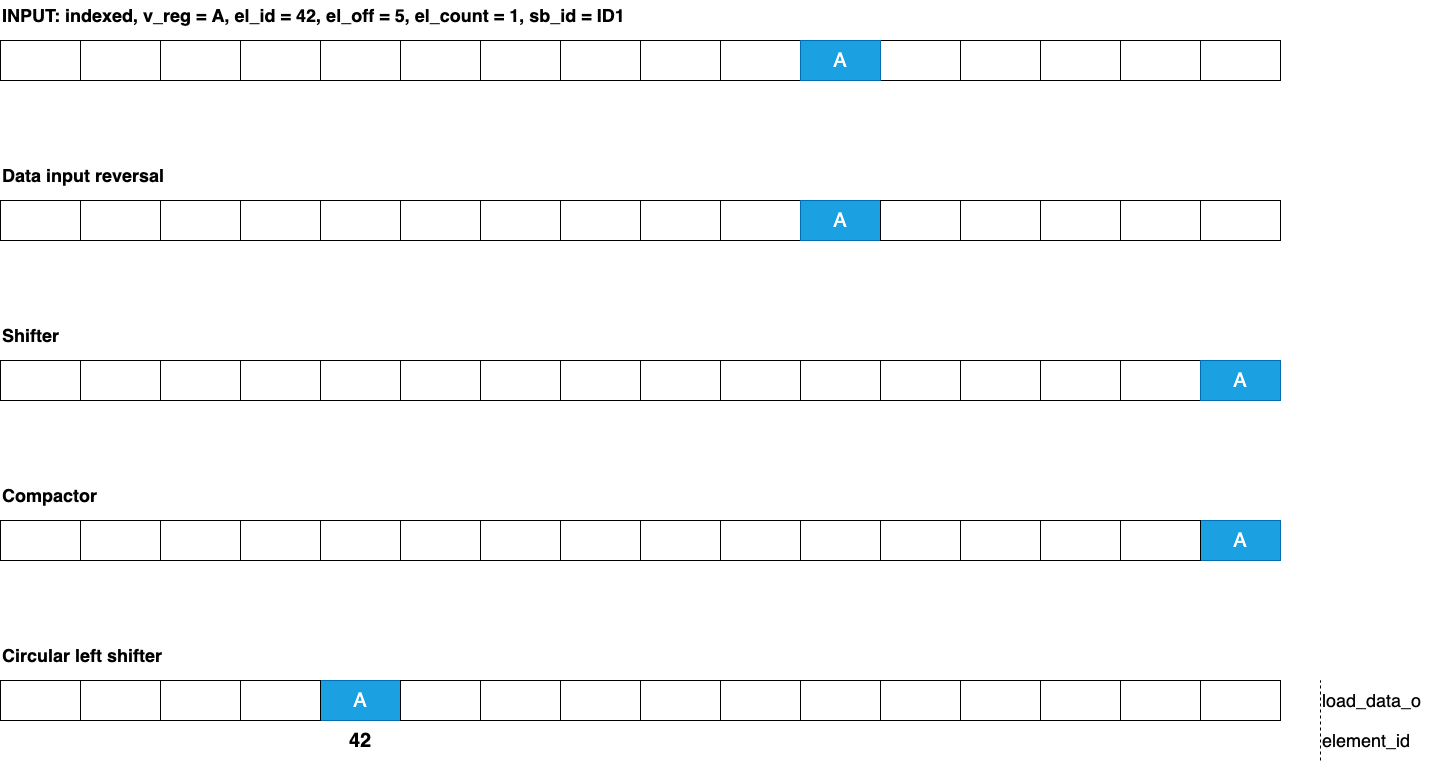
\includegraphics[scale = 0.25]{Chapter_2/img/lmu-indexed.png}
    \caption{Indexed load handled by the LMU}
    \label{lmu-indexed}
\end{figure}

\subsubsection{Masked Load}
All the load operations can be masked. This does not change the number of valid elements, but at the end of the process they will not be sent.\\


In Figure \ref{lmu-masked-stride} it is possible to see an example of the simple strided-load used before, but this time, with a mask.

\begin{figure}[H]
    \centering
    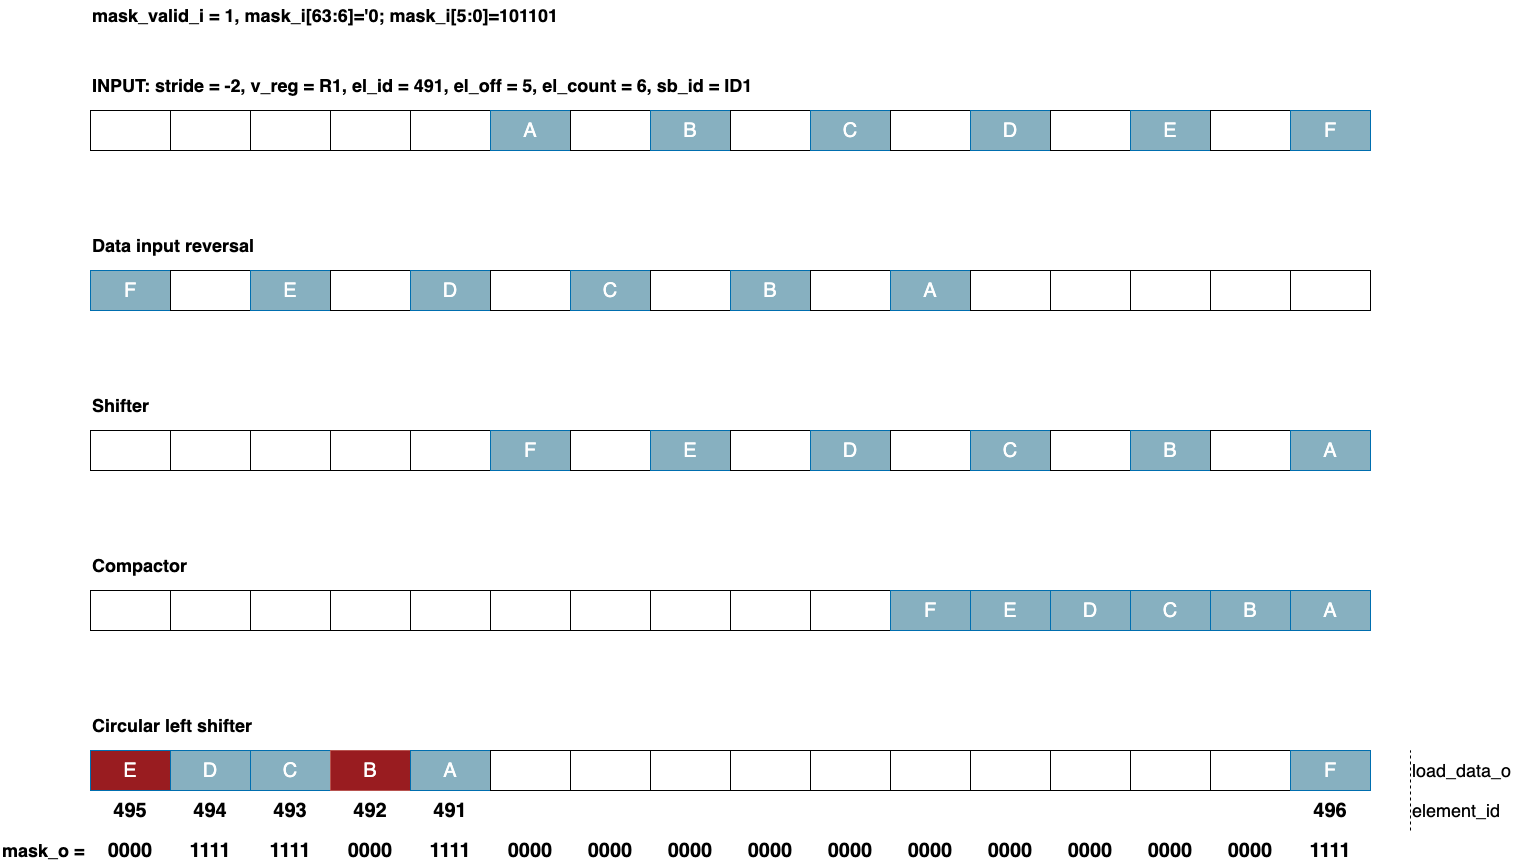
\includegraphics[scale = 0.25]{Chapter_2/img/lmu-masked-strided.png}
    \caption{Strided load, with mask, handled by the LMU}
    \label{lmu-masked-stride}
\end{figure}

\subsection{Load Buffer}
The second submodule that is mainly in charge of the load operation is the Load Buffer.\\
Its function is writing the data sent by Avispado to the Vector Register File. The data can come from different instructions inflight, and the Buffer will always try to optimize and group the data to write.\\

The LMU receives full cache lines of 512 bit from Avispado and forwards them to the corresponding Load Buffer for each lane (64 bit max per lane), depending on the seq\+id\+i. The position of the data into the LB will be determined by the element ID.\\

Up to two loads can be inflight, but their associated cache lines can arrive out-of-order, although the implementation will be parameterized to accept N loads in flight.
\subsubsection{Interface}
The Load Buffer is connected with a lot of modules. From the \emph{Vector Lane} it receives the clock and the reset and communicates if there is a load inflight; with the \emph{LMU} it exchanges all the data; from \emph{Avispado} it knows if the operation has terminated; the requested handshake is handled with the \emph{Memory Queue}; the data goes to the \emph{Vector Register File}, synchronizing with the internal \emph{Finite State Machine}; finally it can commit the result with the \emph{Commit Unit}.\\

A simple connection structure is represented in Figure \ref{lb-if}.

\begin{figure}[H]
    \centering
    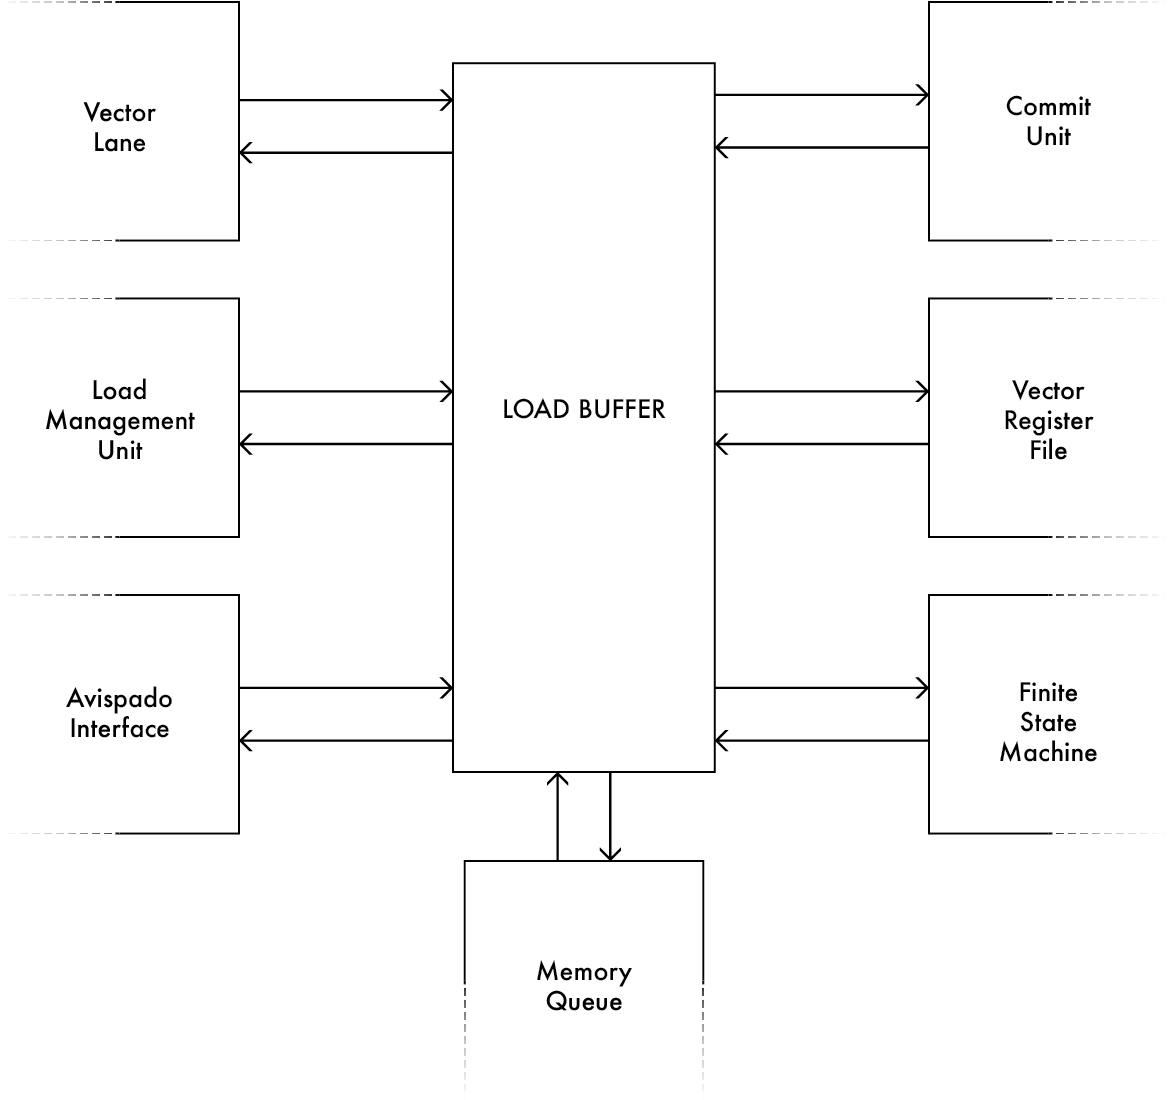
\includegraphics[scale = 0.6]{Chapter_2/img/lb-if.png}
    \caption{Load Buffer's interfaces}
    \label{lb-if}
\end{figure}

\subsubsection{Structure}
There is a Load Buffer of each lane and there are 3 layers to buffer the elements. The layers are divided by the concept of Element Group. In fact, the elements cannot be disposed in every combination, but every element, based on its element ID, has an exact location (based also on the SEW). The position  of the elements follows the structure of the VRF explained in the first Chapter.\\

In Figure \ref{gen-ex} it is possible to see a general connection between the LMU and the various Load Buffers.\\

\begin{figure}[H]
    \centering
    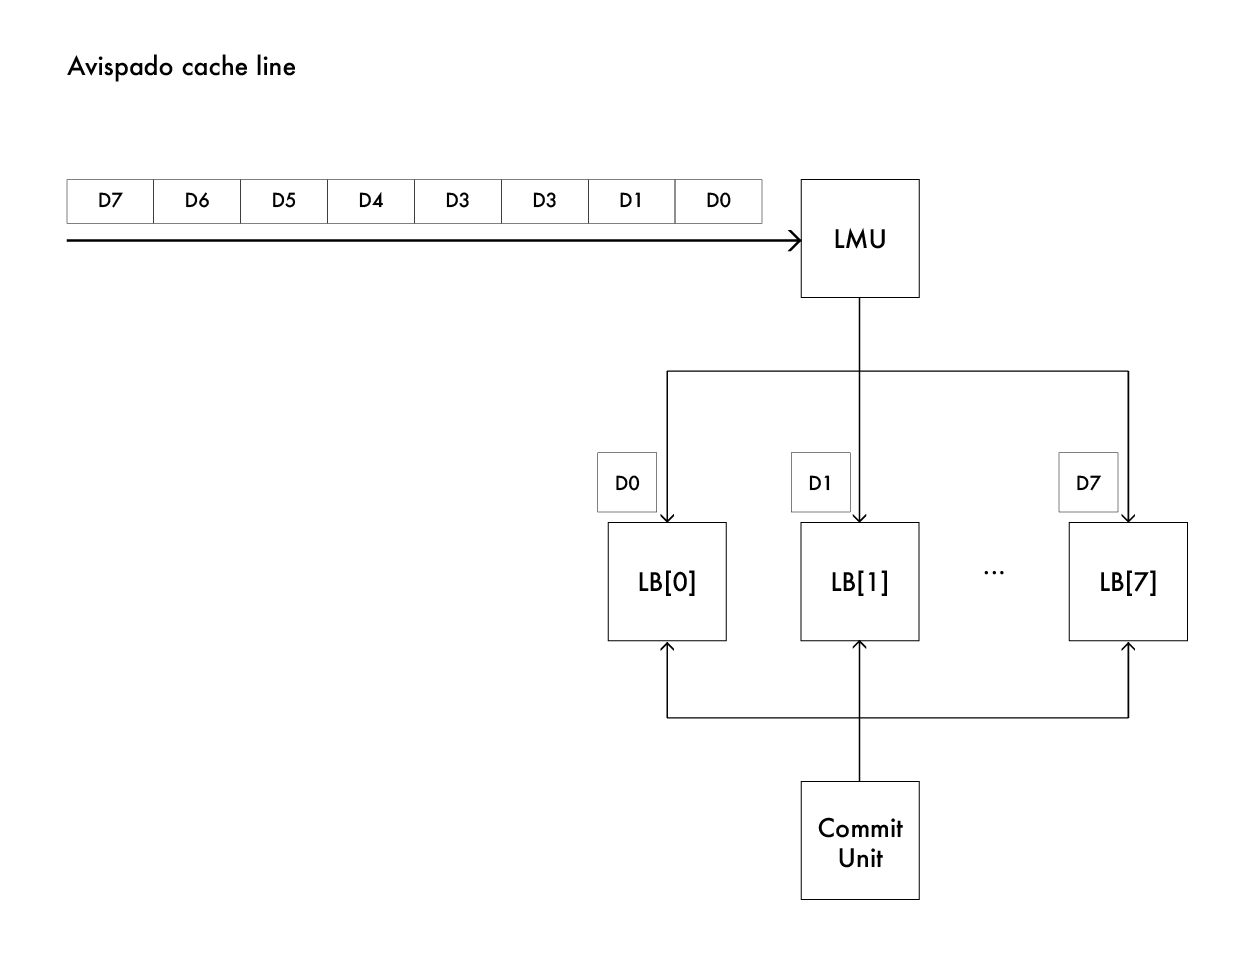
\includegraphics[scale = 0.5]{Chapter_2/img/cache-to-lb-gen-ex.png}
    \caption{Data through the LB}
    \label{gen-ex}
\end{figure}


In Figure \ref{lb-genz} there is an example for the disposition of the elements of 64 bit. It is also important to say that the number of bits for each element group stays the same, this means that the number of elements depends on the SEW.\\


\begin{figure}[H]
    \centering
    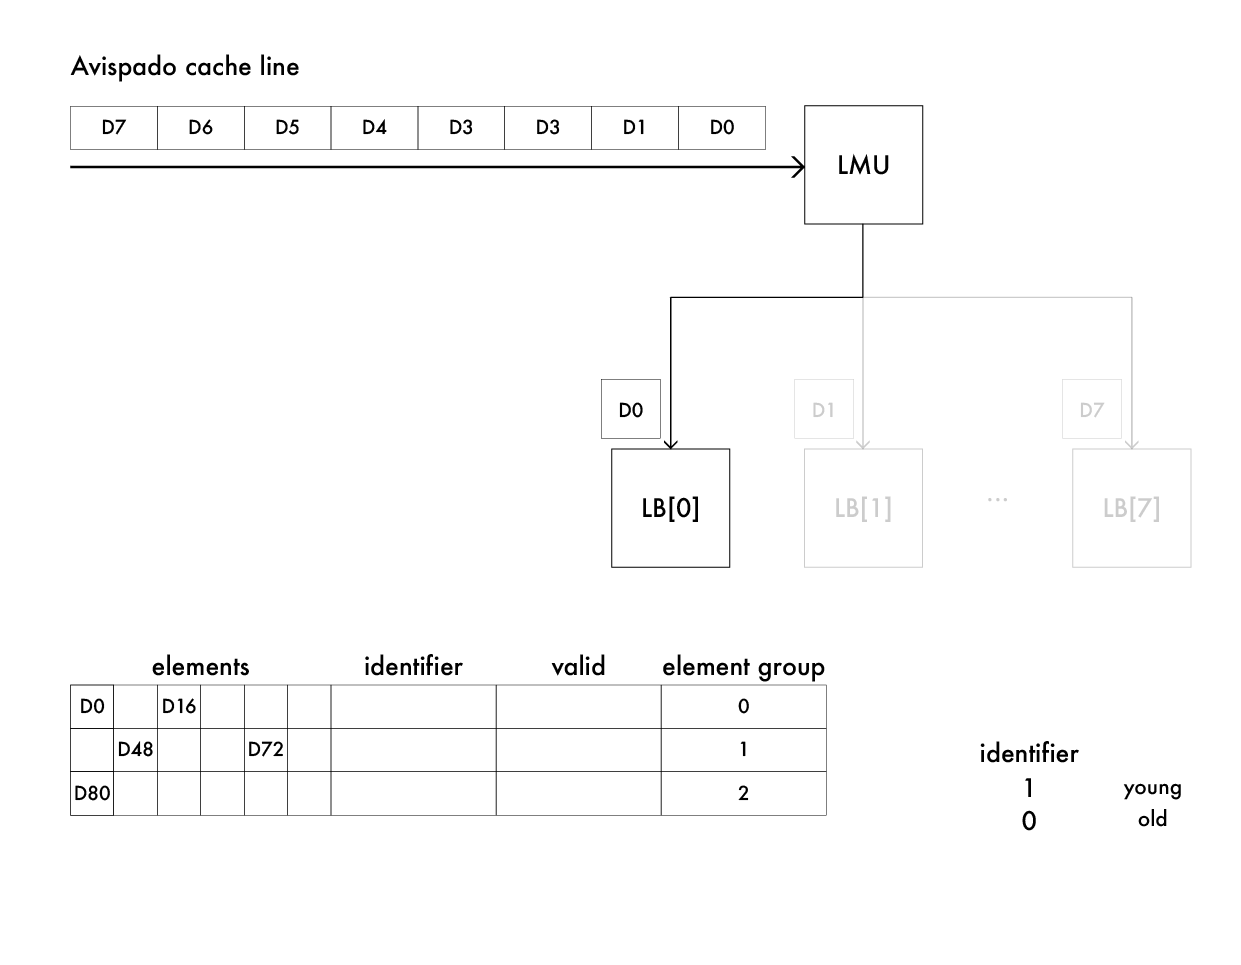
\includegraphics[scale = 0.4]{Chapter_2/img/cache-to-lb-genz-ex.png}
    \caption{General case for the LB}
    \label{lb-genz}
\end{figure}

The Load Buffers are mainly composed of 4 parts:
\begin{itemize}
    \item \emph{Elements}: the elements in the buffer, they are always 512 bit, so 5 elements with SEW = 64, 10 elements with SEW = 32 and so on;
    
    \item \emph{Identifier}: identifies the elements coming from the young or the old load;
    
    \item \emph{Valid}: identifies if the elements are valid;
    
    \item \emph{Element Group}: identifies the group of elements into the Vector Register File. 
\end{itemize}

\subsubsection{Retry}
There are cases in which three buffers are not enough to store all the elements. It is possible that more than three elements try to occupy the same position and so they can cause a problem.\\

This case is handled with a retry mechanism:\\
one of the elements is discarded and a new request is made to Avispado, to notify the retry.\\

Is important to understand the element to discard when there is a retry, whether it is a new or an old one.\\

There are 4 possible cases:
\begin{enumerate}
    \item if the incoming data comes from the \emph{young load} and the buffer does only contain \emph{data from the same load}, it will be discarded the data with the highest element group;
    
    \item if the incoming data comes from the \emph{young load} and the buffer contains \emph{data from both the oldest and youngest loads}, it will discard the incoming data;
    
    \item if the incoming data comes from the \emph{old load} and the buffer only contains \emph{data from the same load}, it will be discarded the data with the highest element group;
    
    \item if the incoming data comes from the \emph{old load} and the buffer contain \emph{data from both the oldest and youngest loads}, it will discard the data inside the buffer, the one from the young load.
\end{enumerate}



\subsubsection{Flow}
In Figure \ref{lb-flow} it is possible to see a simple scheme of the LB's behaviour.

\newpage
\begin{figure}[H]
    \centering
    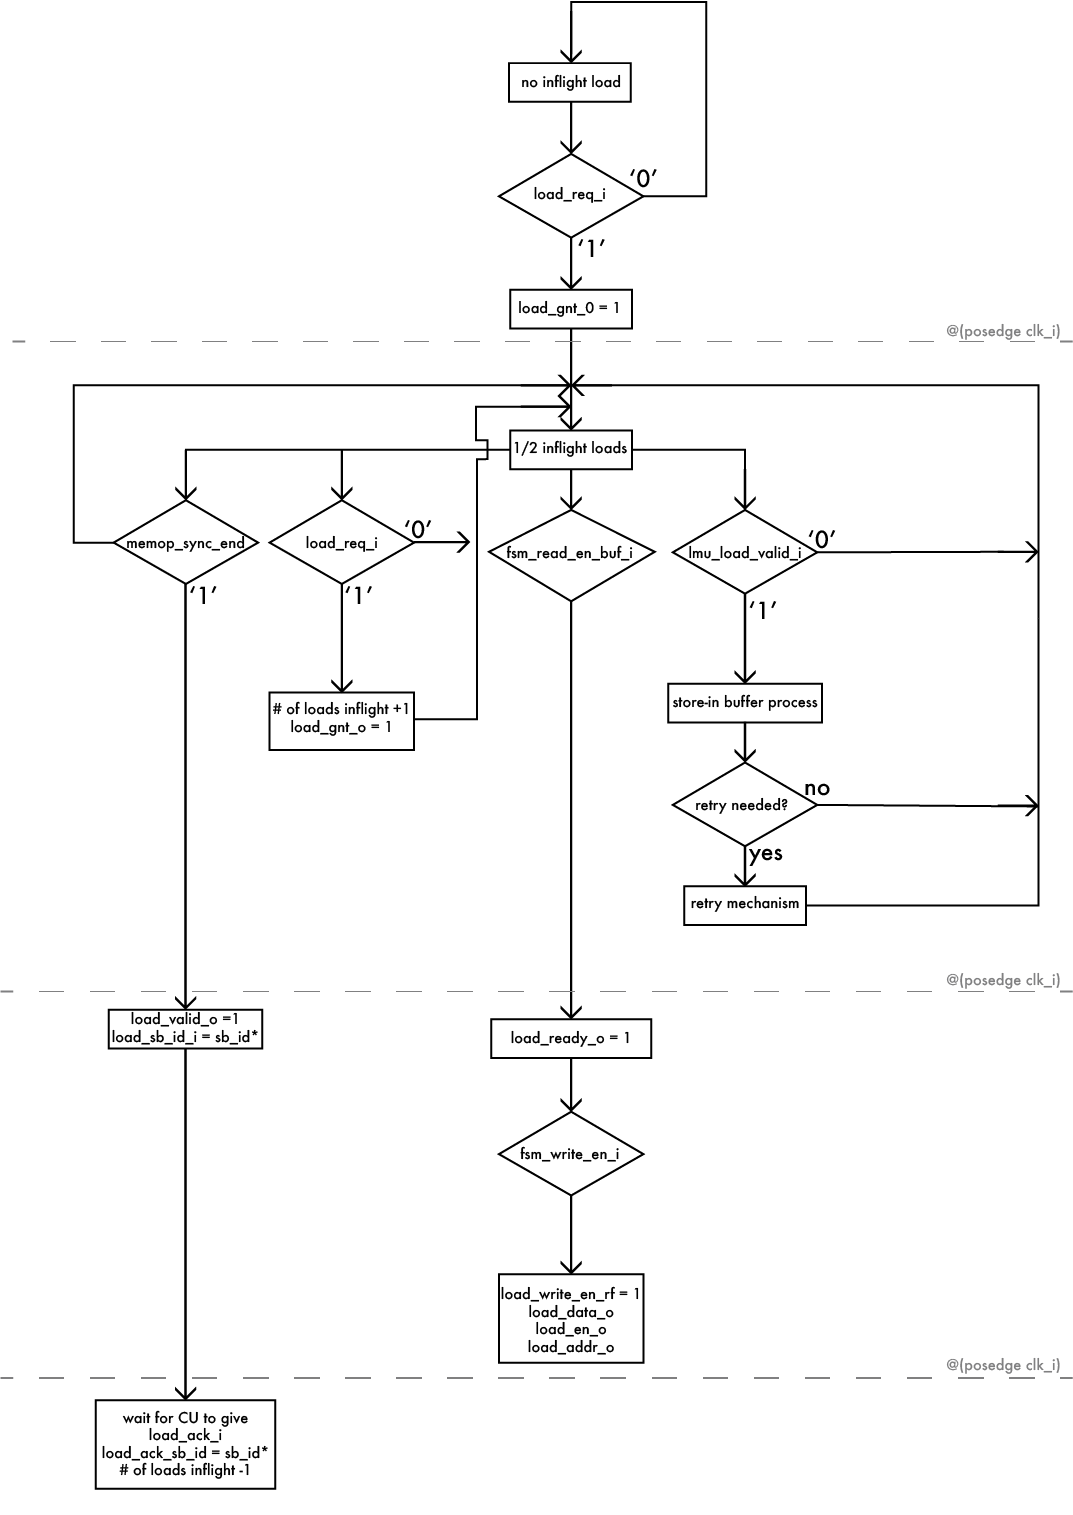
\includegraphics[scale = 0.8]{Chapter_2/img/lb-flow.png}
    \caption{Working flow of the Load Buffer}
    \label{lb-flow}
\end{figure}

Following the scheme it is possible to understand the main working flow of the Load Buffer.\\
When it receives a request it can grant it if the number of load inflight is less than two.\\
For each request the LB can receive the data, and in case activate the retry mechanism, or it can receive a \emph{memop\+sync\+end} and then continue the process to finish the load.\\
During this process it is possible \emph{fsm\+read\+en\+buf\+i} arrives and the LB can write the data in output.\\


\section{Verification Plan}
In order to have a better approach with the verification of a design, it is important to define a Verification Plan.\\
There are many ways to write it. In this specific case, the Verification Team was working along with the Design Team to produce better specifications and not only to test the completed design. This means that the Verification Plan is done following the general rules to have a good value in future, but it is not entirely defined a priori.\\

It was previously defined to create the UVM structure led to the development of all the tools for the verification. \\
Defining the approach to have does also mean defining the tools that will be used, in fact, many different of them were created, such as an \textbf{UVM}, \textbf{checkers} for 
%%TODO



\subsection{Test Plan}
In order to have a good coverage of the cases, and good reports to find bugs, it is very important to have a test plan.\\

The test plan defines all the different cases to test for a submodule or for the entire VPU. This means trying to find all the different corner cases stimulating the DUT.\\

If there is the possibility a good test plan only includes different sets of stimulus, in this way an easy implementation is possible. But this situation does not cover all the possible cases. For instance, not every case could be tested in a submodule of the VPU only modifying the inputs from the scalar core.\\
Which means that sometimes it is necessary to create some modified settings, to create the correct environment for the test.\\

It was created a test plan to stress the load operations. Those are affecting a lot of submodules of the VPU, but the focus will be on the Load Buffer and on the LMU, mainly.\\
Let's now analyze some of the created tests.

\subsubsection{test on consecutive elements}
The first test planned was a simple test about consecutive elements, this means all the elements are sent in order. Of course this is a simple case, and it is thought to test if all the chain to the effective load are working. In fact, it is a regression test.\\

The only constraint meant to be in this test is the sequentiality of the elements.\\
An example could be the one represented in Figure \ref{cache-to-lb-seq-ex}.


\begin{figure}[H]
    \centering
    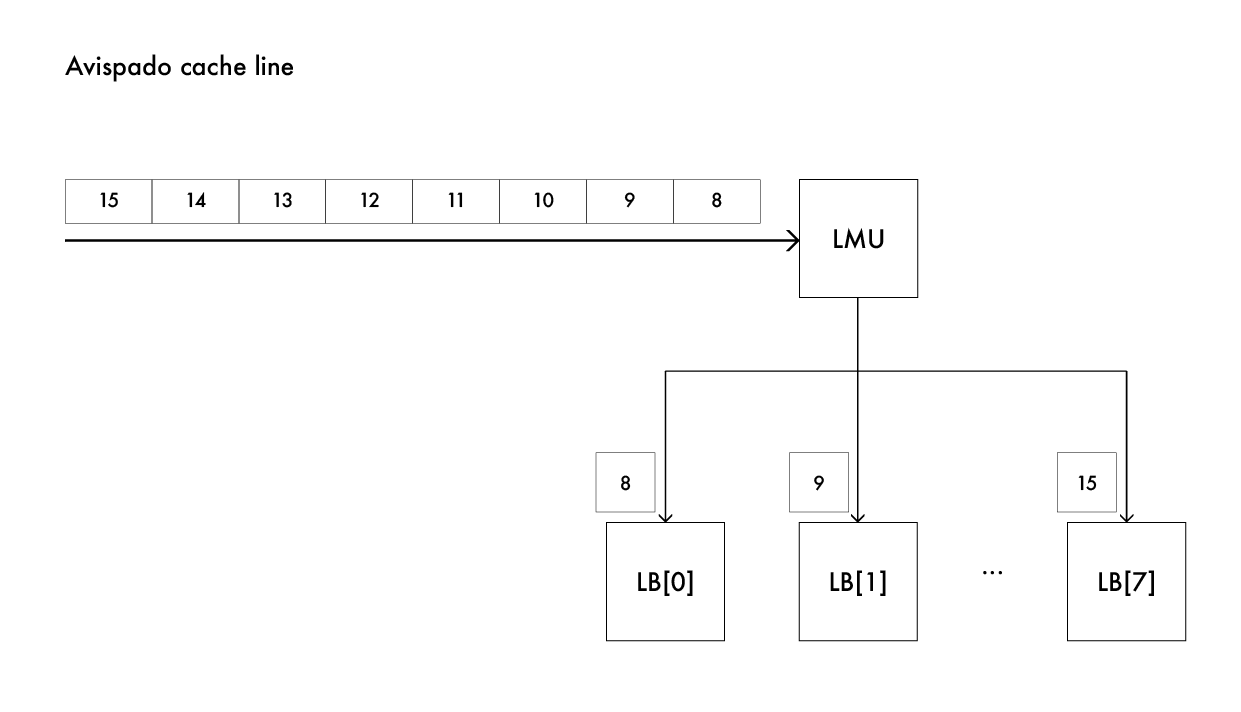
\includegraphics[scale = 0.6]{Chapter_2/img/cache-to-lb-seq-ex.png}
    \caption{Sequential inputs from avispado}
    \label{cache-to-lb-seq-ex}
\end{figure}

\subsubsection{test on random values}
The second kind of test to implement is for sure the random test. This will stress the ability to use different elements ID and different loads at the same time. In this way all the handling for the positions, calculated based on the load and on the element ID, is stressed.\\

It was created a special modality to constrain the randomness to the possible values. This was implemented in the UVM using the configurations for the sequence.\\

An example on random inputs from the same load could be the one represented in Figure \ref{cache-to-lb-rnd-ex}.

\begin{figure}[H]
    \centering
    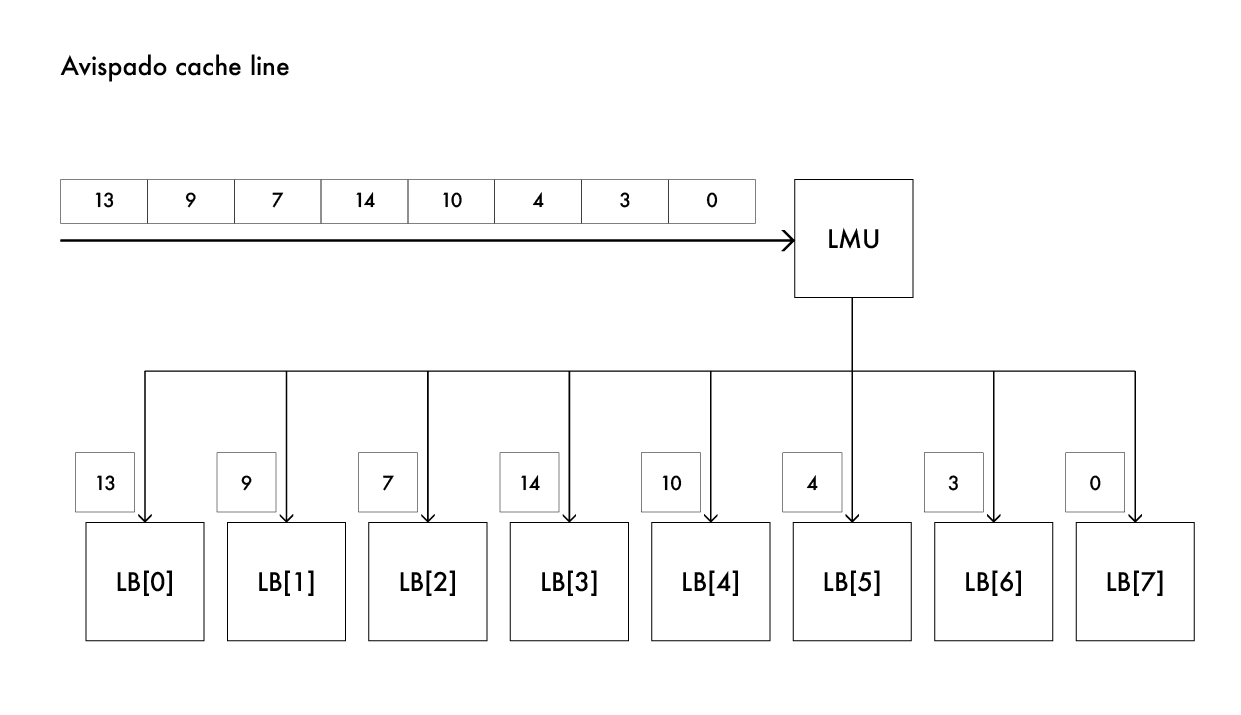
\includegraphics[scale = 0.6]{Chapter_2/img/cache-to-lb-rnd-ex.png}
    \caption{Random inputs from avispado}
    \label{cache-to-lb-rnd-ex}
\end{figure}

It is also possible to have inputs from two loads, as in Figure \ref{cache-to-lb-ooo-ex}.

\begin{figure}[H]
    \centering
    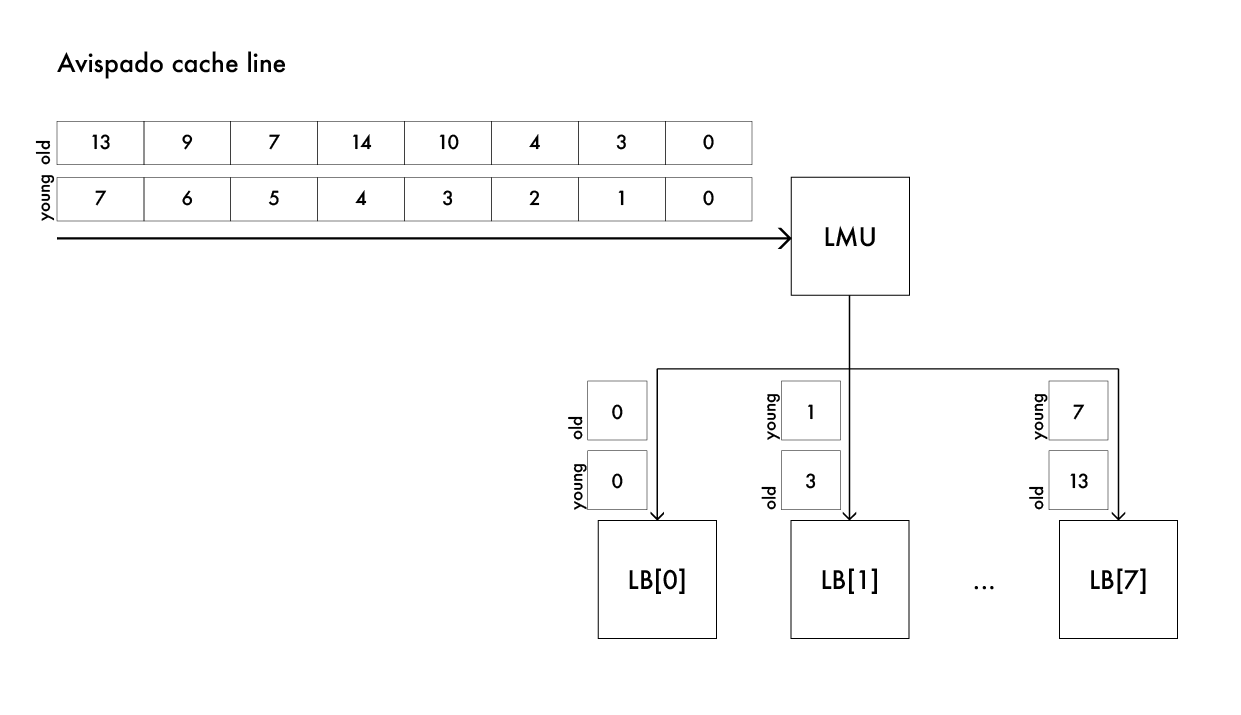
\includegraphics[scale = 0.6]{Chapter_2/img/cache-to-lb-ooo-ex.png}
    \caption{Random inputs from two loads}
    \label{cache-to-lb-ooo-ex}
\end{figure}

\subsubsection{test on splitted elements} 
A very interesting case is revealed when studying the positions.\\
Let's take into account a line of elements sent by the LMU to the Load Buffer. In this case the SEW needs to be different from 64, so the case will use SEW = 32.\\

The data sent will be sequential starting from 65 to 80. In this way it is possible to test if the output is disposed correctly and so if the Load Buffer for the Lane[0] stores 80-65 as values, in this order.\\

An example could be the one represented in Figure \ref{cache-to-lb-split-ex}. It also shows how the input is splitted in the LB.

\begin{figure}[H]
    \centering
    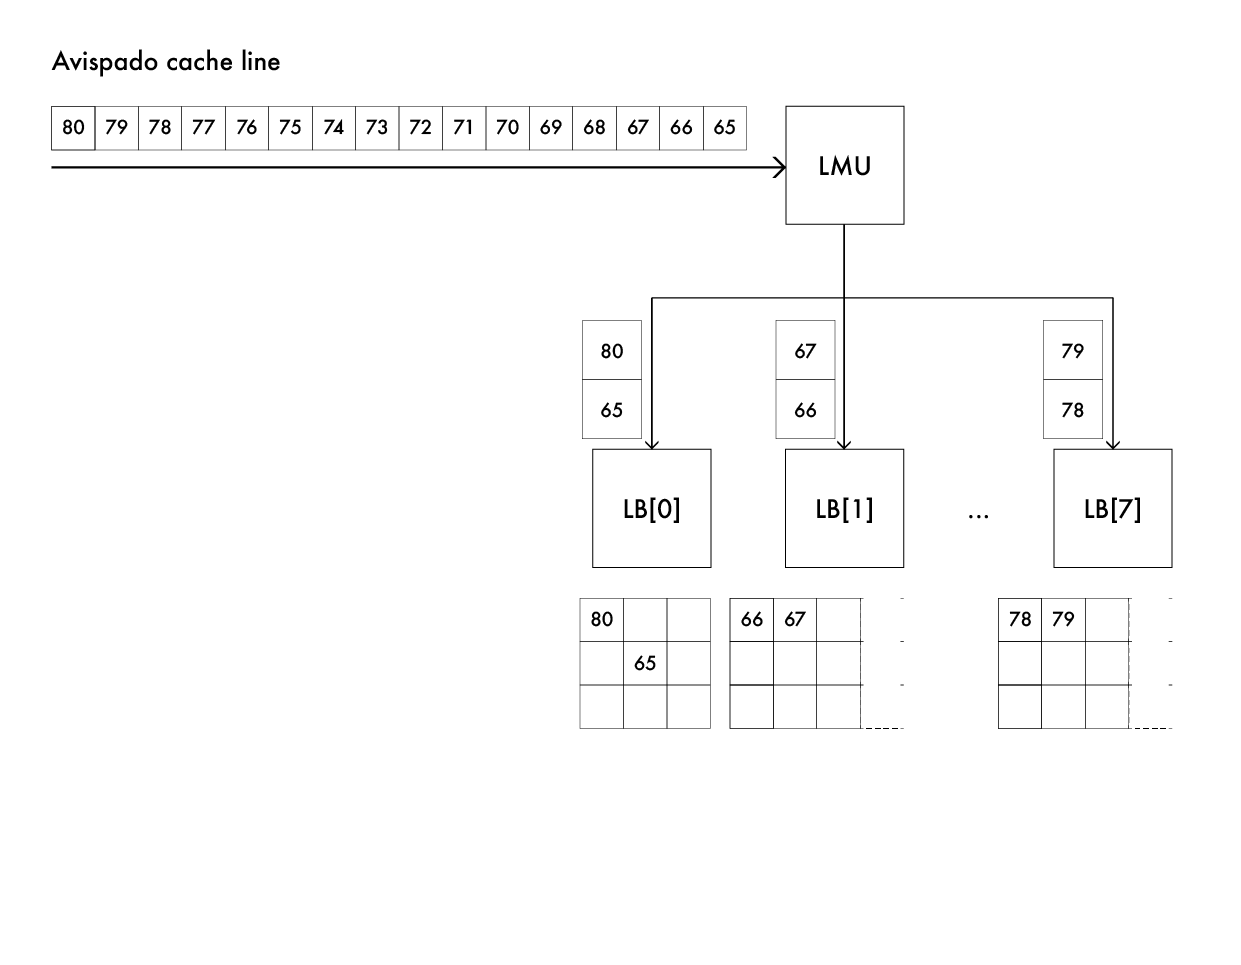
\includegraphics[scale = 0.6]{Chapter_2/img/cache-to-lb-split-ex.png}
    \caption{Input splitted into the LB}
    \label{cache-to-lb-split-ex}
\end{figure}

For reference let's analyze a binary used for this specific case.
\newpage

\linespread{1}
\begin{lstlisting}[language=Verilog,style=verilog-style, backgroundcolor=\color{lyel_palette}, frame=tl]
#define __riscv_xlen 32
#include "test_macros.h"

.globl _start
.section .text

INIT_TEST(e32, 512)

la x1, init_region
addi x1, x1, 0x3c
vle.v v0, 0(x1)


END_TEST

# Initializes 4 registers (256 elements of 64 bit each one)
# TODO Do a macro that allocates N registers...
RVTEST_DATA (
	.dword 0x0000000200000001, 0x0000000400000003; \
	.dword 0x0000000600000005, 0x0000000800000007; \
	.dword 0x0000000A00000009, 0x0000000C0000000B; \
	.dword 0x0000000E0000000D, 0x000000100000000F; \
	.dword 0x0000001200000011, 0x0000001400000013; \
	.dword 0x0000001600000015, 0x0000001800000017; \
        .dword 0x...
        .dw...  

     
 

        
\end{lstlisting}
\linespread{1.2}

The test is initialized with a macro, defining the SEW = 32 and the size in bit = 512.\\
Then the data (the one that follows the instructions) is loaded into a register as address, and is summed an offset of \emph{0x3c}, equal to 60 in decimal.\\ This is the exact value needed to have the first sent element id = 65. As the number of elements will be 512/32 = 16 the element ids will go from 65 to 80.\\

\subsubsection{test on retries}
The last test typology is about the retry mechanism. This occurs when all the three lines are filled with an element in the same position, and then a fourth elements arrives, this means that the Load Buffer does not have another position for one of the elements, thus one of the elements needs to go back to the sender and a new request is made.\\

Considering SEW = 64, there are different versions about this test: it can be a simple in order retry with elements 0-40-80-120-... as inputs, it can be out of order as 0-40-120-80-..., or it can be with two different loads.\\

The easy example is represented in Figure \ref{cache-to-lb-ret-ex}. 0-40-80 are already filling the spots where 120 will try to fit. So a retry is needed, discarding 120.

\begin{figure}[H]
    \centering
    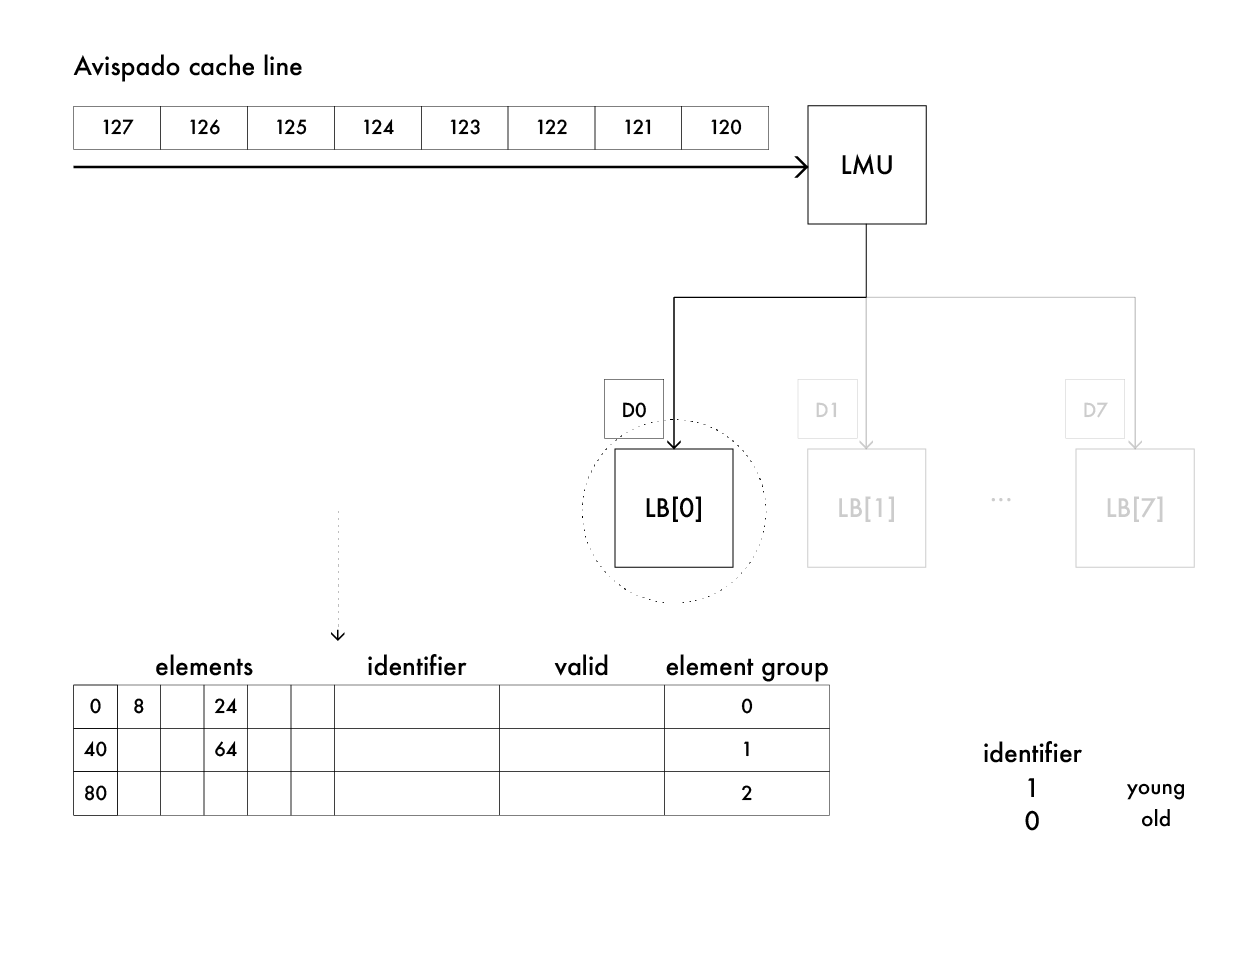
\includegraphics[scale = 0.5]{Chapter_2/img/cache-to-lb-ret-ex.png}
    \caption{Stimulated retry}
    \label{cache-to-lb-ret-ex}
\end{figure}


The out-of-order example is represented in Figure \ref{cache-to-lb-ooo-ret-ex}. 0-40-120 are already filling the spots where 80 will try to fit. So a retry is needed, discarding 120, and taking 80.

\begin{figure}[H]
    \centering
    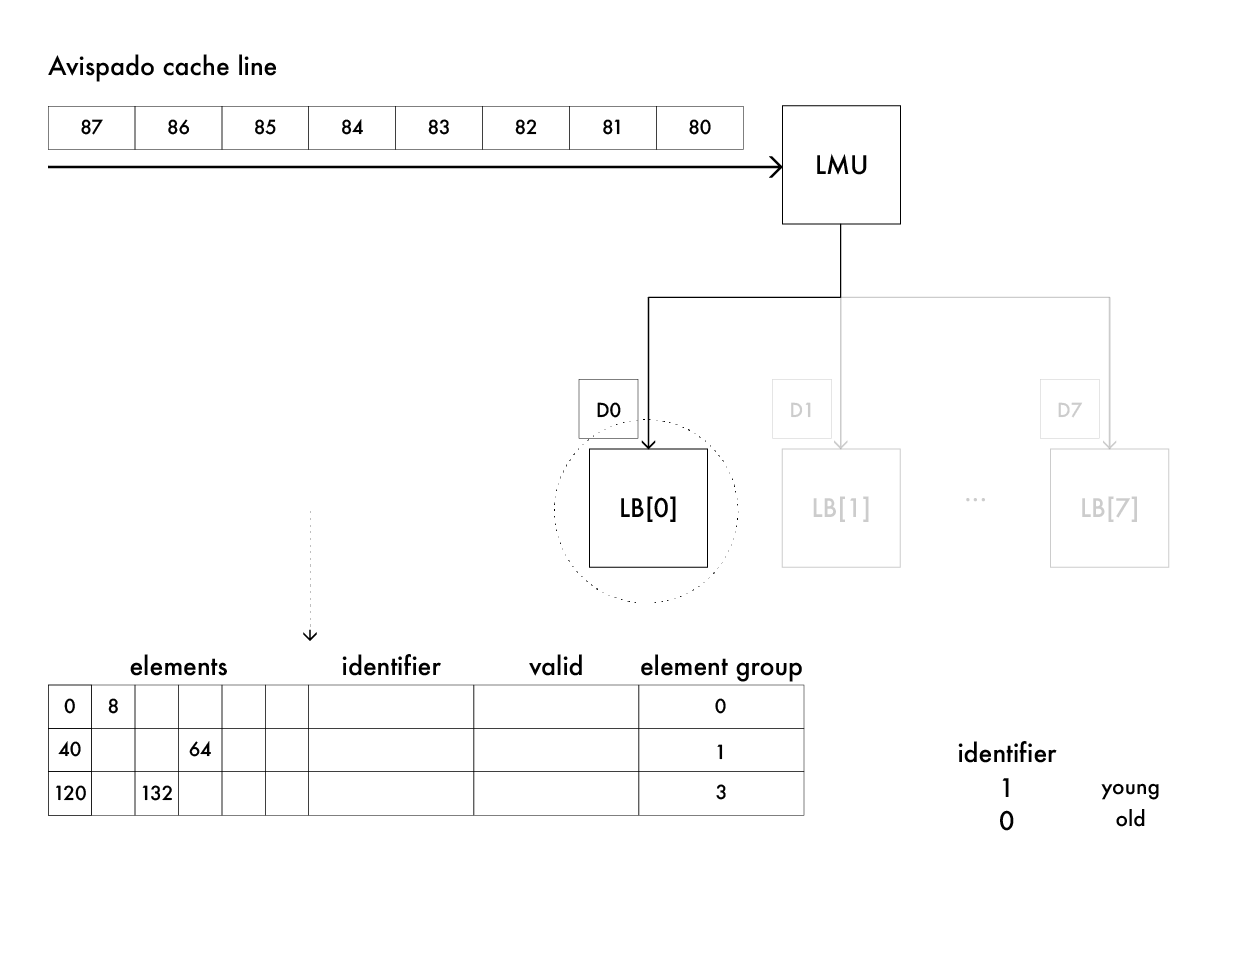
\includegraphics[scale = 0.5]{Chapter_2/img/cache-to-lb-ooo-ret-ex.png}
    \caption{Stimulated retry with out-of-order values}
    \label{cache-to-lb-ooo-ret-ex}
\end{figure}



\section{Verification Process}
The test executed are just the base for the verification. The tests can only define some functionalities, but to test all of them a complete functional verification is required.\\


The approach is normally to define some functionalities and then compare them to the design. This of course is the crucial part, because it is not always obvious how a specific case works. Also there are different ways to test those functionalities.\\

\subsection{Scoreboard}
As saw into the test plan, an easy way to test the results is the scoreboard, thus to have a predicted value and then to compare it against the calculated one.\\

Before the work of this thesis started the UVM for the interface and a scoreboard for the results were already implemented by the BSC verification team. Let's now analyze a little bit how the scoreboard works and why it was useful to develop other tests.

\subsubsection{Spike}
Spike is a RISC-V ISA Simulator. For this specific project it was extended to support the vector extension.

It is used first to simulate the Avispado core, producing stream of vector instructions and memory addresses. Those are feed to the VPU using the UVM. A result is produced using also the Spike vector extension simulation. Finally the results are compared and reported into a scoreboard. A simple scheme is represented in Figure \ref{bin-to-log}.

\begin{figure}[H]
    \centering
    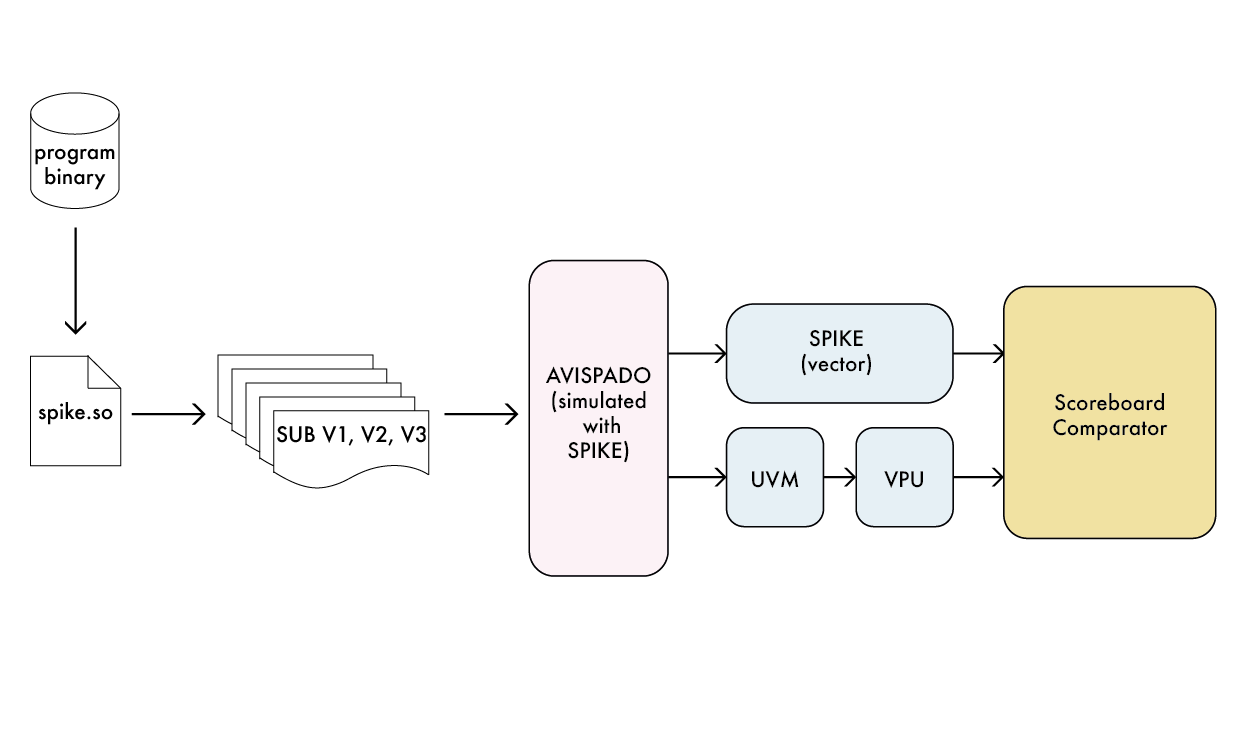
\includegraphics[scale = 0.6]{Chapter_2/img/bin-to-log.png}
    \caption{Simulation path}
    \label{bin-to-log}
\end{figure}

This kind of tool is very useful when running tests because it is faster than a specific test for each component the test is stressing, and at the same time can give hints about the working condition. Of course it is just a first step, because it will be hard to find a bug using only the comparison with the final result.

\subsubsection{Load Management Unit's scoreboard}
The aim of this thesis was principally based on testing the Load operations, so a scoreboard for the LMU was created.

Recalling the LMU working model, it first takes into account the stride, reversing the data in case of negative stride, then the data is positioned correctly again, then it is compacted considering the stride, and finally it is aligned to match with correct ID.

In high level it was done using vectors, and a couple of steps were merged together. It is possible to see below the pseudo code representing the implementation in this way.

\linespread{1}
\begin{lstlisting}[language=Verilog,style=verilog-style, backgroundcolor=\color{lyel_palette}, frame=tlb]
        x=new[N_ELEMENTS][SEW];
        y=new[N_ELEMENTS][SEW];

        //first assignement
        x[N_ELEMETS][SEW] = load_data_i[N_ELEEMTS*SEW]

        //consider the stride
        if(stride<0 && !is_indexed)
            y[i] = x[-i];
        else
            y[i] = x[i];
        

        //from # of bytes to # of elements
        local_stride = mod(local_stride * 8 / SEW);

        //concatenate the data according to stride 
        x[N_ELEMENTS-1-i] = y[(N_ELEMENTS-1-i*local_stride-OFFSET)%N_ELEMENTS];

        //shift the data according to EL_ID
        k = EL_ID % N_ELEMENTS;
        
        y[(N_ELEMENTS-1-(k+i))%N_ELEMENTS] = x[(N_ELEMENTS-1-i)]
\end{lstlisting}
\linespread{1.2}

Also the mask was predicted in a similar way, thus the masking step was then implemented with a simple check on the mask to have the correct result.

In this way it is possible to have an exact result for the LMU, so when a test fails, it is always possible to check if the LMU performed correctly with the data it received in input.

\subsubsection{Load Buffer's scoreboard}
For the Load Buffer the behaviour was really complicated, so a simplified  version of a scoreboard was implemented.

Hence it does not work on the correct result operation per operation, this because the LB has 3 layer of deepness and always tries to optimize the output. So to implement all the rules about the output would be to create a similar structure with an high risk to create a bug in the Verification model.

The concept was to see the data in input and then to expect, eventually, the same data in the correct position as output. This of course is not conflicting with the concept of retry, in fact when a retry is executed it is guaranteed all the data as output, eventually.

It was implemented as an assertion (whose behavior will be explained in the following section), to create a time correlation.

A pseudo version of this checker is represented below.
\bigskip

\linespread{1}

\begin{lstlisting}[language=Verilog,style=verilog-style, backgroundcolor=\color{lyel_palette}, frame=tlb]
// Pseudo checker
if( lmu_dvalid_load_i) { 

    load_data_o[get_el_bank(el_id_i, sew_i)*SEW + SEW-1 -: SEW] == data_i;
}


// This function computes the bank of an element
function [BANK_IDX_SZ-1:0] get_el_bank([EL_ID_WIDTH-1:0] el_id,
            [SEW_WIDTH-1:0] sew);
            
    case (sew[1:0])
        SEW64: get_el_bank=((el_id/N_LANES)%N_BANKS); 
        SEW32: get_el_bank=(((el_id>>1)/N_LANES)%N_BANKS); 
        SEW16: get_el_bank=(((el_id>>2)/N_LANES)%N_BANKS); 
        SEW8:  get_el_bank=(((el_id>>3)/N_LANES)%N_BANKS); 
    endcase
endfunction

\end{lstlisting}

\linespread{1.2}
\bigskip

Using the element\+id and the corresponding bank (based on the SEW), it is possible to predict the result for a specific location and compare it. In this pseudo code it is not very visible the time handling, but the \emph{if} statement will wait until the result goes as output.


\subsection{Checkers}
In order to connect them to the whole structure the binding method was used: basically, when a file containing the checker is created, it is compiled with a bind option to connect it to an RTL file. In this way the files can be kept separate and the Design Team and the Verification Team can work together on different files. \cite{binding}

\begin{lstlisting}[language=Verilog,style=verilog-style, backgroundcolor=\color{lyel_palette}, frame=l, numbers=none]
$PATH_LB/LoadBuffer.sv -mfcu -cuname $PATH_LBC/LoadBuffer_checker.svh
\end{lstlisting}
spiegazione
%TODO
\begin{lstlisting}[language=Verilog,style=verilog-style, backgroundcolor=\color{lyel_palette}, frame=l, numbers=none]
bind LoadBuffer LoadBuffer_checker bind_LoadBuffer_checker (.*);
\end{lstlisting}


\subsubsection{Load Management Unit's assertions}
The main focus was on the calculated result and on the handshake with the other components.

In the verification plan were previously defined all the functionality to check, then a list of assertions was used to produce a good checker.

The list of all the checkers can be found in Appendix.

\begin{table}[H]
    \centering
    \begin{tabular}{|l|l|}
    \hline
    
    \hline
    
   \lgray \textbf{name} & \lgray \textbf{functionality} \\ \hline
   
   \hline
   
\toran a\+el\+count & when load\+data\+valid\+i \\ \toran  & then $seq\_id[28:22] (el\_count) \leq \frac{( n\_elements - el\_offset )}{(stride*8/sew)}$ \\ \hline

\tloran a\+stride \+i & $stride\cdot8$ can be one of the following $\pm{} (sew, 2\cdot sew,  4\cdot sew)$ \\\tloran & with SEW = $2^{(3+sew)}$ and not indexed load \\ \hline

\toran a\+load\+granted\+i\+known & when load\+granted\+i, \\ \toran & not unknown the following : SEW, granted\+sb\+id \\ \hline

\tloran a\+load\+data\+i\+known & when data\+valid\+i, \\\tloran & not unknown seq\+id\+i, load\+data\+i \\ \hline

\toran a\+sb\+id\+o & when load\+data\+valid\+i ,\\\toran & next clock cycle sb\+id\+o(t) = seq\+id\+i[29:32](t-1) \\ \hline

\tloran a\+load\+dvalid\+o\+known \tloran & when load\+dvalid\+o, outputs known \\ \hline

\toran a\+dvalid\+o & after load\+data\+valid\+i,\\\toran & next clock cycle, load\+dvalid\+o \\ \hline

\tloran a\+vstart\+o & correct v\+start\+next\+o v\+start\+self\+o, \\\tloran &  according to load\+data\+o \\ \hline

\toran a\+granted\+ids & can not be granted 2 loads with the same id at once \\ \hline

\tloran a\+indexed\+instr & when the load is an indexed load, \\\tloran & el\+count=1 and mask\+valid\+i = 0 \\ \hline

\toran a\+load\+sync\+end\+i & for every load\+granted\+i \\\toran & there is eventually the corresponding load\+sync\+end\+i  \\ \hline

\tloran a\+load\+grant\+beh & when num\+load\+inflight = 2, load\+grant\+i = 0 \\ \hline

\toran a\+load\+sync\+end\+beh & when num\+load\+inflight = 0, load\+sync\+end\+i = 0 \\ \hline

\tloran a\+load\+req\+sync\+end & load\+sync\+end\+i cannot be simultanous with a load\+granted\+i \\ \hline

\toran a\+el\+count\+sew\+i & when $stride\_i \neq (1, 2, 4)\cdot sew\_i$ (in bytes), \\\toran & el\+count has to be = 1 \\ \hline

\hline

\tlazzu a\+sb\+correct & when load\+dvalid\+i, \\\tlazzu & if it is given a sb\+id not present in the fifo,\\\tlazzu &  load\+dvalid\+o will be 0 \\\hline

\tazzu a\+data\+o & correct load\+data\+o, \\\tazzu & clk cycle after load\+dvalid\+i (stride/mask/indx)\\\hline

\tlazzu a\+mask\+o & correct mask\+o, according to load\+data\+o\\\hline

\tazzu a\+el\+ids\+o & correct element\+ids\+o\\\hline

\tlazzu a\+min\+el\+id\+idx\+o & correct min\+el\+id\+idx\+o\\\hline

\hline

\tyel a\+rsn\+o & when rsn\+i load\+dvalid\+o = 0 and mask\+o = '0 \\\hline
\tlyel a\+rsn\+i & when rsn\+i load\+data\+valid\+i = 0 \\ \tlyel & and load\+granted\+i = 0 \\\hline

    \end{tabular}
    \caption{Assertions on LMU}
    \label{tab_lmu_check}
\end{table}

As it is possible to see in Table \ref{tab_lmu_check} there are different assertions possible for a single submodule. 
Here they are separated by colour distinguishing the different "categories".
Indeed the red ones are checking the basic signals behaviour and the handshakes.\\
An example is \textbf{a\+dvalid\+o}:
\bigskip

\linespread{1}

\begin{lstlisting}[language=Verilog,style=verilog-style, backgroundcolor=\color{lyel_palette}, frame=tlb]
property p_dvalid_o;
	@(posedge clk_i)
	load_data_valid_i && sb_correct |-> ##1 load_dvalid_o ;
endproperty : p_dvalid_o



a_dvalid_o : assert property( disable iff(!rsn_i || kill_i) p_dvalid_o ) 
        else $error('LMU did not compute any output');

\end{lstlisting}
\linespread{1.2}
\bigskip
\begin{itemize}
    \item \textbf{load\+data\+valid\+i} is the input necessary to fire the assertion;
    
    \item \textbf{sb\+correct} is the result of a task, that calculates if the scoreboard\+id is a valid one;
    
    \item \textbf{| - >} is the separation between the firing condition and the checking one. It is not time consuming (the time consuming version would be | = >), so checking for the second condition starts immediately;
    
    \item \textbf{\#\#1} command refers to 1 \textit{clock cycle(s)} delay;
    
    \item \textbf{load\+dvalid\+o} asserted is the expected output.
\end{itemize}

The light blue ones are scoreboard-like assertions, indeed are checking the scoreboard\+id, the data in output and also the masks.\\
They use the results of the tasks to check the values, it is possible to see an example in \textbf{a\+el\+ids\+o} is possible to see how an assertion uses the result of a task.

\newpage
\linespread{1}
\begin{lstlisting}[language=Verilog,style=verilog-style, backgroundcolor=\color{lyel_palette}, frame=tlb]
//task
task compute_ids(int unsigned SEW, int unsigned EL_COUNT, 
	    int unsigned EL_ID, int unsigned N_ELEMENTS);

    int unsigned f_v_e, i, j;
		
    // f_v_e is the index of the first 11-bit-element 
    // of computed_el_id_o where we have to put an EL_ID
	f_v_e = EL_ID % N_ELEMENTS; // find the first valid element 
	f_v_e = f_v_e * SEW / 8 ; // multiply it by the number of bytes per el
		
	// initialize to 0
	for(j=0;j<MAX_NUMBER_ELEMENTS;j++) begin
	    computed_el_id_o[j] = '0;
	end

	for(j=0;j<EL_COUNT;j++) begin
		for(i=0;i<SEW/8;i++) begin
			computed_el_id_o[(f_v_e+i+(j*SEW/8))%MAX_NUMBER_ELEMENTS] 
			    = EL_ID+j;
		end
	end

endtask : compute_ids

// property
property p_el_ids_o;
	bit [MAX_NUMBER_ELEMENTS-1:0][EL_ID_WIDTH-1:0] buffer_ids;
	@(posedge clk_i)
	(load_data_valid_i  && sb_correct, buffer_ids = computed_el_id_o)|-> 
        ##1 element_ids_o == buffer_ids;
endproperty : p_el_ids_o

//assertion
a_el_ids_o : assert property( disable iff(!rsn_i || kill_i) p_el_ids_o ) 
        else $error('mismatch in element_ids_o');
\end{lstlisting}
\linespread{1.2}
\bigskip

It is possible to see the property uses the value \textit{computed\+el\+id\+o}, a global variable. It is important to say the task compute\+ids is not called by the property but from another external process not displayed here.

Finally the yellow ones are just checking the conditions for the reset and the expected output.

It is also important to notice, some of those \textit{are not assertions}, but \textit{assumptions}. This means that they are conditions on the input and not on the outputs. There is no difference for the Functional Verification, but there will be for the Formal one. This will be better explained later on this Chapter.



\subsubsection{Load Buffer's assertions}
A similar approach was adopted for the Load Buffer. Having a lot of interfaces the LB has also a lot of handshakes, and so assertions. For this in the Table \ref{tab_lb_check} are only reported some categories containing all the assertions for an interface.


\begin{table}[H]
    \centering
    \begin{tabular}{|l|l|}
    \hline
    
    \hline
    
    \lgray \textbf{name} & \lgray \textbf{functionality} \\ \hline
   
    \hline
   
    \tazzu \textbf{AVISPADO IF} & \tazzu this is the interface with the scalar core\\ \hline
   
    \hline
\tlazzu a\+mem\+sync\+end\+i & if mem\+sync\+end\+i is high, \\\tlazzu & memop\+sb\+id\+i must be a known value \\\hline

\tlazzu a\+valid\+after\+sync\+end & for every memop\+sync\+end\+i (with a valid memop\+sb\+id\+i) \\\tlazzu & there will be a load\+valid\+o (with correct load\+sb\+id\+o)\\\hline

\tlazzu a\+memop\+sync\+end\+num & if num of memop\+sync\+end\+i = num of load\+ack\+i +2, \\\tlazzu  & then only memop\+sync\+end with \\\tlazzu & a sb\+id different from the ones stored\\\hline

\tlazzu a\+load\+ack\+i\+num & if the num of load\+ack\+i is in excess, \\\tlazzu &  we assume this ack is for a different operation\\\hline

\tlazzu a\+unique\+request & there can not be a request with the same sb\+id \\\tlazzu &  of an inflight load\\\hline

    \hline

    \tgre \textbf{LMU INTERFACE} & \tgre from this interface the LB receive the cache lines\\ \hline
   
    \hline

    \hline

    \tyel \textbf{MQ INTERFACE} & \tyel from this interface the load are requested/granted\\ \hline
   
    \hline

    \hline

    \toran \textbf{FSM INTERFACE} & \toran from this interface comes the enable to write on the VRF\\ \hline
   
    \hline

    \hline

    \tpur \textbf{CU INTERFACE} & \tpur to this interface the ids for and ended load are sent\\ \hline
   
    \hline

    \hline

    \tred \textbf{VRF INTERFACE} & \tred this is the interface to load the data\\ \hline
   
    \hline
    
    \tlred a\+load\+inflight & load\+inflight\+o is checked, \\\tlred & it can be 1 when the number of load inflight is 1 or 2 and \\\tlred & it can be 0 otherwise \\ \hline
    
    \tlred a\+load\+ready\+o & when load\+inflight\+o = 1 and lmu\+dvalid\+load\+i = 1, \\\tlred & if there is fsm\+read\+en\+lbuf\+i, \\\tlred & the next clock cycle there is load\+ready\+o = 1 \\ \hline
    
    \tlred a\+data\+corruption & check that each element that enter \\\tlred & will eventually exit in correct position \\ \hline

    \hline

    \tpin \textbf{VL INTERFACE}  & \tpin from this interface the clk and the rst are recived \\ \hline
   
    \hline

    \end{tabular}
    \caption{Assertions on LB}
    \label{tab_lb_check}
\end{table}

A good example for the handshake is \textbf{a\+mem\+sync\+end\+i}. This is an assumption on the inputs, but will be treated as an assertion.\\

\linespread{1}
\begin{lstlisting}[language=Verilog,style=verilog-style, backgroundcolor=\color{lyel_palette}, frame=tlb]
property p_mem_sync_end_i;
	@(posedge clk_i)
	memop_sync_end_i |-> !$isunknown(memop_sb_id_i);
endproperty : p_mem_sync_end_i


a_mem_sync_end_i : assume property (disable iff (!rsn_i || kill_i) p_mem_sync_end_i) 
        else $error('unknown memop scoreboard id on memop_sync_end_i asserted');


\end{lstlisting}
\linespread{1.2}

The property is using the system function \textbf{\emph{\$isunknown}}, this function return if the value passed is unknown ('\emph{X}' or '\emph{Z}'). So basically when \textbf{\emph{memop\+sync\+end\+i}} is asserted, it must be known the value of its scoreboard id.


Then  \textbf{a\+data\+corruption} is the scoreboard like discussed before, and finally there are the reset's ones.
The assertions are reported into the Appendix.




\subsection{Drivers}
The other tool used to test the submodules is the Driver. It is a file that defines the stimuli and their order. A very defined order of them defines an operation. It is so possible to create the situation in which the DUT will work as expected.

It is important to notice the driver is enabled only when the UVM is configured as ACTIVE.

\subsubsection{Load Management Unit}
This is the only submodule on which was developed a driver, due to the reduced complexity. In fact, the driver can be very complex when different handshakes are present.

In the next page it is possible to see one of the operations implemented into the driver, as example.
\newpage
\linespread{1}
\begin{lstlisting}[language=Verilog,style=verilog-style, backgroundcolor=\color{lyel_palette}, frame=tlb]
if(command.op == gnt_op) begin
    // randomizations
    SEW = command.sew_i;
    SEW = (2**(3+SEW))/8; // in number of bytes , for the stride in bytes
    randomize(command.stride_i) 
        with {command.stride_i inside{1*SEW,2*SEW,4*SEW,-1*SEW,-2*SEW,-4*SEW,
        command.n*SEW};};

    randomize(command.load_granted_sb_id_i) 
        with{!(command.load_granted_sb_id_i inside
        {fifo[0].sb_id, fifo[1].sb_id});};

    // check how many inflight load
    if ( !fifo[0].done && !fifo[1].done ) begin
	    @(posedge lmu_if.clk_i) ;
	    lmu_if.load_data_valid_i = 0;
	    lmu_if.load_sync_end_i=1;
	    lmu_if.load_sync_end_sb_id_i=fifo[command.which_load].sb_id;	
	    fifo[command.which_load].done = 1;
    end 

    // driving
    @(posedge lmu_if.clk_i);
    lmu_if.load_sync_end_i=0;
    lmu_if.load_sync_end_sb_id_i='0;
    @(posedge lmu_if.clk_i);
    lmu_if.load_sync_end_i=0;
    lmu_if.load_sync_end_sb_id_i='0;
    lmu_if.op = gnt_op;
    lmu_if.rsn_i = 1'b1;
    lmu_if.kill_i = 1'b0;
    lmu_if.load_granted_i = 1;
    lmu_if.indexed_load_granted_i = command.indexed_load_granted_i;
    lmu_if.load_granted_sb_id_i= command.load_granted_sb_id_i;
    lmu_if.load_data_valid_i = 0;
    lmu_if.load_data_i = '0;
    lmu_if.seq_id_i = '0;
    lmu_if.mask_valid_i = 1'b0;
    lmu_if.mask_i = '0;
    lmu_if.sew_i = command.sew_i;     
    lmu_if.stride_i = command.stride_i;
    // update the fifo
    if ( fifo[1].done ) begin
	    fifo[1].SEW = command.sew_i;
	    fifo[1].STRIDE = command.stride_i;
	    fifo[1].sb_id = command.load_granted_sb_id_i ;
	    fifo[1].is_indexed = command.indexed_load_granted_i;
	    fifo[1].done = 0;
    end
    else if( fifo[0].done ) begin
	    fifo[0].SEW = command.sew_i;
	    fifo[0].STRIDE = command.stride_i;
	    fifo[0].sb_id = command.load_granted_sb_id_i;
	    fifo[0].is_indexed = command.indexed_load_granted_i;
	    fifo[0].done = 0;
    end
    @(posedge lmu_if.clk_i);
    lmu_if.load_granted_i = 0;
    -> lmu_if.new_input;
end




\end{lstlisting}
\linespread{1.2}
\newpage


The operation implemented is the granting of a load request. The code is mainly divided in three parts: 
\begin{itemize}
    \item the \emph{first} one makes some randomization for the data and the checks if the driver is following the assumptions about the inputs (in this case on the loads inflight);
    
    \item the \emph{second} part is the driving part, all the inputs are well defined, and also some clock cycles need to be waited sometimes. All the value assigned with \textbf{\emph{command}} have been randomized, but constrained to valid values;
    
    \item the \emph{third} part is just the updating of an internal fifo, useful to be in sync with the LMU and to not fail the assumptions.
\end{itemize}  
\bigskip








Let's now move on to the results of the functional and formal analysis.

\chapter{Results and Considerations}
In this chapter there will be discussed the results and the material created during all the work of this thesis.\\

It is important to say that the results are not the only parameter defining if a good verification work was done or not. In fact building the infrastructure and create documentation are important tasks that every verification engineer will eventually do, and they will produce results in long term, so it could be possible they are not directly correlated to some found bug.\\


\section{Found Bugs}
The thesis was developed while the design and the specifications were on going and so unstable. To synchronize all the work it was used the GitLab structure, creating issues and discussing the problems. A well defined issue was then assigned to a design engineer to fix it.\\

The majority of the bugs were found on the Load Management Unit. Let's now analyze some of them.\\

\subsubsection{the indexed load bug}
This one is an issue found using the Formal tools and trying to define better specifications for the Load Management Unit.\\

The problem was the following:
The LMU used the sequence\+id, in particular the \emph{el\+count} field, to identify if the load was strided or indexed. In particular, el\+count contains the number of valid elements being loaded; when this value was el\+count = 1 then the load was considered as indexed.\\
The issue was presenting because the indexed load should ignore the stride value, and so there is no way to send only one element with a stride, or better, in this case the load would not ignore the stride, as every operation was actually a strided one.\\

The better solution for this problem was to create a new signal, \emph{is\+indexed}, to identify an indexed load. The stride will be always ignored when this signal is asserted, and the value of el\+count must be = 1.\\

\subsubsection{the load id bug}
This issue regards the load ids. In the first version when a load was finished it was sent to the \emph{load\+sync\+end\+i} signal to notify that a load was finished.\\

It was sent without an identifier to understand which of the two possible loads was finished, so a FIFO was used to end them in order.\\

This was an issue because the loads should have the possibility to end out-of-order, so a new signal was created: \emph{load\+sync\+end\+sb\+id\+i}. This signal is the id that identifies the load to end.\\

This issue was found analyzing the specs to create the Test Plan.

\subsubsection{the out-of-order load bug}
This issue regards the out-of-order loads. In the Load Management Unit there is a FIFO handling the load\+ids for the two possible inflight loads.\\

The FIFO was freed of an element only when another one was put as input. But it could have been possible that an already inflight load was into the FIFO, let's say with id = 1, and another load with id = 1 issued. \\
Having the same id the configurations for the second load would have been overwritten.\\

This issue was found analyzing the result of two consecutive loads, with same id, but one was strided and another one was indexed. The second load was not considered as indexed failing the condition that says el\+count = 1.\\

This was the case of a typical bug finding flow: first the whole big tests fails during a load. Then it is examined using the assertions on the load modules. Exploring the waveform is then possible to find the bug.\\

\subsubsection{the after kill bug}
This bug is related to the validity of the output of the LMU.\\

When there is a kill, the entire instruction needs to be killed. But it could be possible to receive valid data for a killed load. This because the kill mechanism needs some time to stop the operation.\\

So the LMU should ignore the input from a killed instruction, but this was not the case. Indeed the validity of the data in output was assumed every time the data was valid in input.\\

It caused the simulation to time out on the next instruction. This because the kill was not issue correctly, so the starting point for the next instruction was not clean. \\

This issue can represent a valid example of why the formality on the assertions in very important.\\
Consider the following code:\\

\linespread{1}
\begin{lstlisting}[language=Verilog,style=verilog-style, backgroundcolor=\color{lyel_palette}, frame=tlb]
property p_dvalid_o;
@(posedge clk_i)
load_data_valid_i && sb_correct |-> ##1 load_dvalid_o ;
	endproperty : p_dvalid_o

a_dvalid_o : assert property( disable iff(!rsn_i || kill_i) p_dvalid_o )
else $error('LMU did not compute any output');
\end{lstlisting}
\linespread{1.2}

In this case, the assertion is testing if there is \emph{load\+dvalid\+o} when the input is valid. But it does not test if \emph{load\+dvalid\+o} has always a valid \emph{load\+data\+valid\+i} a clock cycle before.\\

The property as reported is not able to spot the error in this issue, but knowing where is the problem is possible to use the correctness of this assertion to understand the problem.\\

\subsubsection{the two loads bug}
This issue was spotted both in the LMU and in the LB. The modules received two loads with the same id. This led to an assumption error, as every load has an unique id.\\

In reality the problem was not in the Load Management Unit nor in the Load Buffer, but in the memory queue. In fact, this modules is the responsible to hand the ids for each load.\\

Also this issue was found so late in the verification process because was depending on a trigger enabled by the kill.\\

For reference in Figure \ref{2-loads} there is the interface of a simulation, in particular on the waveforms. It is possible to see two loads issue with the same id.\\

\begin{figure}[H]
    \centering
    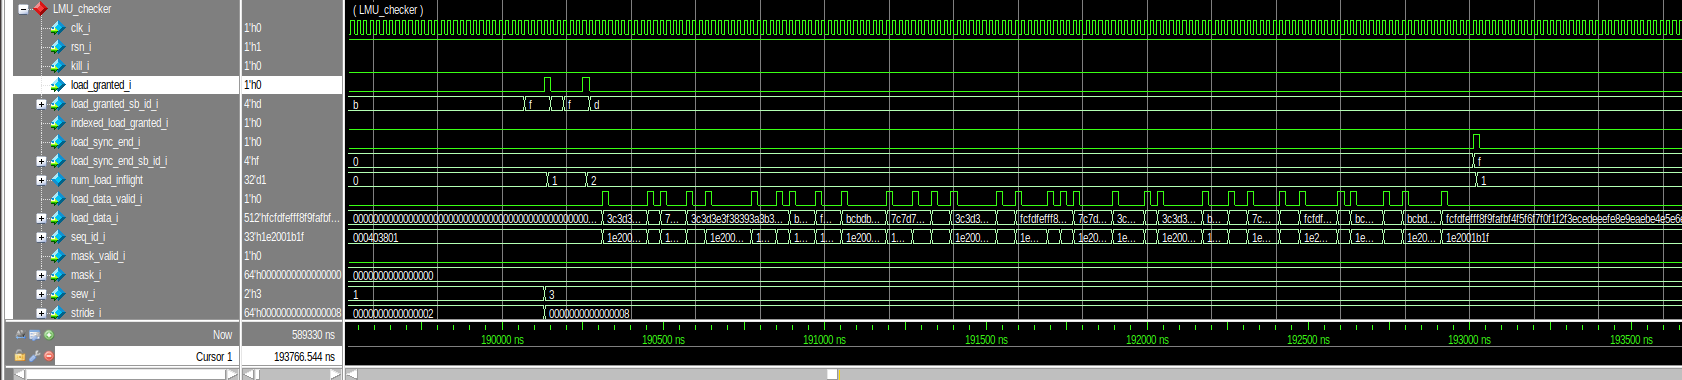
\includegraphics[scale = 0.25]{Chapter_3/img/2-loads.png}
    \caption{Two loads issued with ther same id}
    \label{2-loads}
\end{figure}


\section{Material Created}
Other than the found bugs there is also some material created during this thesis.\\
In particular on the structure to handle the test of the submodules.\\

\subsubsection{UVM}
A complete UVM was created, to drive and test the Load Management Unit. It has also the possibility to have different tests with different sequences and so constraints.\\

\linespread{1}
\begin{lstlisting}[language=Verilog,style=verilog-style, backgroundcolor=\color{lyel_palette}, frame=tlb]
class lmu_constrained_test extends lmu_random_test;
    `uvm_component_utils(load_management_unit_constrained_test)

	function void build_phase(uvm_phase phase);
		lmu_sequence_item::type_id::
		  set_type_override(lmu_constrained_sequence_item::get_type());
		super.build_phase(phase);
	endfunction


	function new(string name, uvm_component parent);
      		super.new(name,parent);
   	endfunction : new


endclass : lmu_constrained_test
\end{lstlisting}
\linespread{1.2}
In this code the base\+test is extended and then it is overridden into the build\+phase the sequence\+item.\\
\linespread{1}
\begin{lstlisting}[language=Verilog,style=verilog-style, backgroundcolor=\color{lyel_palette}, frame=tlb]
class lmu_constrained_sequence_item extends lmu_sequence_item;
	`uvm_object_utils(lmu_constrained_sequence_item)

	constraint few_rst{op dist{rsn_op:=1,gnt_op:=5,load_op:=9,kill_op:=2};}
	

	function new(string name = "");
		super.new(name);
	endfunction : new

endclass : lmu_constrained_sequence_item
\end{lstlisting}
\linespread{1.2}
In the sequence new constraints are applied. In this case the probability for the operation are defined.\\

This kind of structure is very reusable and expandable, also and it can be improved during the whole verification process.\\

\subsubsection{specifications}
Other than that some documentation was created, on missing specifications and on guides to perform certain kinds of checks. This is very important during a project because allows the other members to partecipate actively.\\

This work was not done in one shot, but required a looped check on the behaviour obtained. The specs and the design were still being developed, this means also the documentation should have been. But this was not always the case, so a constant check (helped also with the formal tool, very useful to define the correct assumptions) helped to maintain the documentation correct.\\

\subsubsection{verification plan}
The verification plan was half prepared when the work of this thesis started. However when starting the creation of the checkers a lot of changes were upcoming, so important modifications were done to the test plan. It was also done following a standard to avoid incompatibilities when using it with other software.\\
The assertion reported into the Appendix are following the verification plan implemented.\\

\subsubsection{test plan}
The test plan for the loads was entirely created during the process of this thesis. It required first some confidence with the load operation, then it was possible to update the simple cases and fill it with interesting corner cases.\\

In order to give validity to the test plan it was important to create an easy way to run those tests. For that were done some configurable modalities.\\


\subsubsection{modalities}
The last contribution was to create the modalities for the implemented tests. Such modalities are way to stimulate the VPU modifying some settings into the UVM. This allows to order the data in specific ways or to force some mechanism inside the VPU. In the code below it is possible to see a couple of them.\\

\linespread{1}
\begin{lstlisting}[language=Verilog,style=verilog-style, backgroundcolor=\color{lyel_palette}, frame=tlb]
//(for beautiness there is also a subtraction in case of overflow, 
//in order to start from the smallest index possible).
//The range_id is NOT getting smaller as the overflow occurs, 
//because we do not want to cause more retries, so we put the index fixed to 0

else if (m_cfg.seq_id_mode == RETRY_ID) begin
    if(loop_ooo[load_index] <= 3 & loop_ooo[load_index] > 0) begin
        range_id[load_index] = c_lines_per_group -1 ;
        seq_id_index[load_index] = (seq_id_index[load_index] +
            range_id[load_index])%(inflight_loads[load_index].seq_ids.size());
            
    end
    else seq_id_index[load_index] = 0;
        loop_ooo[load_index] += 1;
        
end


//Here we want to stimulate 0-40-120-80 id seq, 
//so we choose the correct cycle value and manipulated the range.
//then the cycle after the range returns to be 4 and stale.

else if (m_cfg.seq_id_mode == RETRY_OOO_ID) begin
    if(loop_ooo[load_index] == 0) begin
        range_ooo_id[load_index] = c_lines_per_group - 1;
        seq_id_index[load_index] = 0;

    end else begin
        if(loop_ooo[load_index] == 3) 
            range_ooo_id[load_index] = 2*range_ooo_id[load_index] + 1;
        if(loop_ooo[load_index] == 4) 
            range_ooo_id[load_index] = -(c_lines_per_group);
        if(loop_ooo[load_index] == 5) 
            range_ooo_id[load_index] = c_lines_per_group -1;
        seq_id_index[load_index] = (seq_id_index[load_index] +
            range_ooo_id[load_index])%(inflight_loads[load_index].seq_ids.size());
        if(loop_ooo[load_index] > 5) 
            seq_id_index[load_index] = 0;
    end
    loop_ooo[load_index] += 1;
end



\end{lstlisting}
\linespread{1.2}

It is possible to see the handling of the element id sent by avispado. In this case it is manipulated the order of the ids, and this will not cause an error as the final result will be the same.\\

In this way it is possible to stimulate the retry mechanism sending all the elements for the same position into the Load Buffer. There is also another version for the out-of-order retry.\\

Those modalities can be configured for each test, and so randomized. In this way they can be implemented in the automatic tests.

\chapter{Conclusions}
\section{Conclusions}
Starting from the concepts of the vector extensions and then the VPU it was possible to understand why this kind of parallel processing is gaining more and more relevance nowadays.\\

In this thesis was shown all the effort done to verify the behaviour of some DUTs, in particular for the load operations.\\

The first one was the Load Management Unit, and it was shown its mechanism to send the data to the buffers. This complexity resolved in a lot of issues during the design, in fact a lot of techniques were applied.\\
It was explained how drive a component by itself, extrapolating it from a structure, helps to understand its blind spots.\\
Very crucial was the correct defining of a Verification Plan, that allowed to create an high level model to be used as scoreboard.\\
The verification plan was also important to better define the specifications and, as saw in the founded issues, to add or remove signals were necessary.\\

The second one was the Load Buffer, which required a different approach. It was too complex to create a complete scoreboard. However it was still possible to create an sort of scoreboard divided in more assertions, predicting the majority of the cases without introducing new errors.\\
It was also very important define a Test Plan, stressing all the corner cases for the storing of the data. This also required an easy way to be implemented, so it was created as binary file combined with some modalities created ad-hoc.\\

Finally all the results were presented, explaining some of the most common issue that can be founded.\\
It was also very important the contribution on the documentation created and on the structure provided to test the submodules. Indeed this UVM is standalone and was designed to be launched with some simple command launching the correct script.\\

Thanks to all those techniques it was possible to go on with the design reducing the number of people needed to check for all the bugs.\\

\section{Future developments}
Regarding the verification process, there is still some space for future developments. In particular the next steps would be to complete the Verification Plan and add assertions and assumption for all the submodules. This will require a little bit of time, but then it will be very easy to add the coverage monitoring. \\

Talking about the entire project, it is now important to catch up with the specifications that are being updated by RISC-V. In this way it will be possible to provide an innovative VPU, very useful to be implemented in HCP.
\chapter{Appendix}
\UseRawInputEncoding
\lstset{breaklines} 
\lstset{showstringspaces=false} 
\section{Checkers}
\subsection{Load Buffer} 
\lstinputlisting[language=Verilog,style=verilog-style]{./Appendix/LoadBuffer_checker.svh}

\subsection{Load Management Unit} 
\lstinputlisting[language=Verilog,style=verilog-style]{./Appendix/load_management_unit_checker.svh}



\begin{appendix}
  \listoffigures
  \listoftables
\end{appendix}

\newpage

\bibliographystyle{ieeetr}
\bibliography{mybib}

%nocite{*}




\end{document}






